\mfpicnumber{1}

\opengraphsfile{Relations}

\setcounter{footnote}{0}

\label{Relations}

From one point of view,\footnote{Carl's, of course.} all of Precalculus can be thought of as studying sets of points in the plane.  With the Cartesian Plane now fresh in our memory we can discuss those sets in more detail and as usual, we begin with a definition.

\medskip

\colorbox{ResultColor}{\bbm

%\smallskip

\begin{defn}

\label{relatonsdefn}

A \index{relation ! definition} \textbf{relation} is a set of points in the plane.

%\smallskip

\end{defn}

\ebm}

\medskip

Since relations are sets, we can describe them using the techniques presented in Section \ref{SetsofNumbers}.  That is, we can describe a relation verbally, using the roster method, or using set-builder notation. Since the elements in a relation are points in the plane, we often try to describe the relation graphically or algebraically as well.  Depending on the situation, one method may be easier or more convenient to use than another.  As an example, consider the relation $R = \{ (-2,1),(4,3), (0,-3) \}$.  As written, $R$ is described using the roster method.  Since $R$ consists of points in the plane, we follow our instinct and plot the points.  Doing so produces the  \index{graph ! of a relation} \textbf{graph} of $R$.

\begin{center}

\begin{mfpic}[19]{-5}{5}{-5}{5}
\point[4pt]{(-2,1),(4,3), (0,-3)}
\tlabel[cc](-2,1.5){$(-2,1)$}
\tlabel[cc](4,2.5){$(4,3)$}
\tlabel[cc](1.25,-3){$(0,-3)$}
\axes
\tlabel[cc](5,-0.5){\scriptsize $x$}
\tlabel[cc](0.5,5){\scriptsize $y$}
\xmarks{-4,-3,-2,-1,1,2,3,4}
\ymarks{-4,-3,-2,-1,1,2,3,4}
\tcaption{The graph of $R$.}
\tlpointsep{5pt}
\scriptsize
\axislabels {x}{{$-4 \hspace{7pt}$} -4, {$-3 \hspace{7pt}$} -3, {$-2 \hspace{7pt}$} -2, {$-1 \hspace{7pt}$} -1, {$1$} 1, {$2$} 2, {$3$} 3, {$4$} 4}
\axislabels {y}{{$-4$} -4, {$-3$} -3, {$-2$} -2, {$-1$} -1, {$1$} 1, {$2$} 2, {$3$} 3, {$4$} 4}
\normalsize
\end{mfpic}

\end{center}

In the following example, we graph a variety of relations.

\begin{ex}  Graph the following relations. \label{relationgraphingexample}

\begin{multicols}{2}
\begin{enumerate}

\item  $A = \{ (0,0), (-3,1), (4,2), (-3,2)\}$
\item  $HLS_{\mbox{\tiny$1$}} = \{ (x,3) \, | \, -2 \leq x \leq 4\}$

\setcounter{HW}{\value{enumi}}
\end{enumerate}
\end{multicols}

\begin{multicols}{2}
\begin{enumerate}
\setcounter{enumi}{\value{HW}}

\item  $HLS_{\mbox{\tiny$2$}} = \{ (x,3) \, | \, -2 \leq x < 4\}$ \label{opencircleintroduction}
\item  $V = \{ (3,y) \, | \, \mbox{$y$ is a real number} \}$

\setcounter{HW}{\value{enumi}}
\end{enumerate}
\end{multicols}

\enlargethispage{.25in}
\vspace{-.15in}

\begin{multicols}{2}
\begin{enumerate}
\setcounter{enumi}{\value{HW}}

\item  $H = \{ (x,y) \, | \, y = -2 \}$
\item  $R = \{ (x,y) \, | \, 1 < y \leq 3 \}$

\setcounter{HW}{\value{enumi}}
\end{enumerate}
\end{multicols}
\vspace{-.2in}

\pagebreak

{\bf Solution.}  

\begin{enumerate}

\item  To graph $A$, we simply plot all of the points which belong to $A$, as shown below on the left.

\item  Don't let the notation in this part fool you.  The name of this relation is $HLS_{\mbox{\tiny$1$}}$, just like the name of the relation in number 1 was $A$.  The letters and numbers are just part of its name, just like the numbers and letters of the phrase `King George III' were part of George's name.  In words,  $\{ (x,3)\, | \, -2 \leq x \leq 4 \}$  reads `the set of points $(x,3)$ such that $-2 \leq x \leq 4$.'   All of these points have the same $y$-coordinate, $3$, but the $x$-coordinate is allowed to vary between $-2$ and $4$, inclusive.  Some of the points which belong to $HLS_{\mbox{\tiny$1$}}$ include some friendly points like:  $(-2,3)$, $(-1,3)$, $(0,3)$, $(1,3)$, $(2,3)$, $(3,3)$, and $(4,3)$.  However, $HLS_{\mbox{\tiny$1$}}$ also contains the points $(0.829, 3)$, $\left(-\frac{5}{6}, 3\right)$, $( \sqrt{\pi}, 3)$, and so on.  It is impossible\footnote{Really impossible.  The interested reader is encouraged to research \href{http://en.wikipedia.org/wiki/Countable_set}{\underline{\textbf{countable}}} versus \href{http://en.wikipedia.org/wiki/Uncountable_set}{\underline{\textbf{uncountable}}} sets.} to list all of these points, which is why the variable $x$ is used.  Plotting several friendly representative points should convince you that $HLS_{\mbox{\tiny$1$}}$ describes the horizontal line segment from the point $(-2,3)$ up to and including the point $(4,3)$.

\hspace{.25in} \begin{tabular}{m{2.7in}m{2.7in}}

\begin{mfpic}[18]{-5}{5}{-1}{5}
\point[4pt]{(0,0),(-3,1), (4,2), (-3,2)}
\axes
\tlabel[cc](5,-0.5){\scriptsize $x$}
\tlabel[cc](0.5,5){\scriptsize $y$}
\xmarks{-4,-3,-2,-1,1,2,3,4}
\ymarks{1,2,3,4}
\tlpointsep{5pt}
\scriptsize
\axislabels {x}{{$-4 \hspace{7pt}$} -4, {$-3 \hspace{7pt}$} -3, {$-2 \hspace{7pt}$} -2, {$-1 \hspace{7pt}$} -1, {$1$} 1, {$2$} 2, {$3$} 3, {$4$} 4}
\axislabels {y}{{$1$} 1, {$2$} 2, {$3$} 3, {$4$} 4}
\normalsize
\tcaption{The graph of $A$}
\end{mfpic} & 

\begin{mfpic}[18]{-5}{5}{-1}{5}
\polyline{(-2,3), (4,3)}
\point[4pt]{(-2,3),(4,3)}
\axes
\tlabel[cc](5,-0.5){\scriptsize $x$}
\tlabel[cc](0.5,5){\scriptsize $y$}
\xmarks{-4,-3,-2,-1,1,2,3,4}
\ymarks{1,2,3,4}
\tlpointsep{5pt}
\scriptsize
\axislabels {x}{{$-4 \hspace{7pt}$} -4, {$-3 \hspace{7pt}$} -3, {$-2 \hspace{7pt}$} -2, {$-1 \hspace{7pt}$} -1, {$1$} 1, {$2$} 2, {$3$} 3, {$4$} 4}
\axislabels {y}{{$1$} 1, {$2$} 2, {$3$} 3, {$4$} 4}
\normalsize
\tcaption{The graph of $HLS_{\mbox{\tiny$1$}}$}
\end{mfpic} \\

\end{tabular}

\item  $HLS_{\mbox{\tiny$2$}}$ is hauntingly similar to $HLS_{\mbox{\tiny$1$}}$.  In fact, the only difference between the two is that instead of `$-2 \leq x \leq 4$' we have `$-2 \leq x < 4$'. This means that we still get a horizontal line segment which includes $(-2,3)$ and extends to $(4,3)$, but we do \emph{not} include $(4,3)$ because of the strict inequality $x < 4$.   How do we denote this on our graph?  It is a common mistake to make the graph start at $(-2,3)$ end at $(3,3)$ as pictured below on the left.  The problem with this graph is that we are forgetting about the points like $(3.1, 3)$, $(3.5, 3)$, $(3.9, 3)$, $(3.99, 3)$, and so forth.  There is no real number that comes `immediately before' $4$, so to describe the set of points we want, we draw the horizontal line segment starting at $(-2,3)$ and draw an open circle at $(4,3)$ as depicted below on the right.

\hspace{.25in} \begin{tabular}{m{2.7in}m{2.7in}}

\begin{mfpic}[18]{-5}{5}{-1}{5}
\polyline{(-2,3), (3,3)}
\point[4pt]{(-2,3),(3,3)}
\axes
\tlabel[cc](5,-0.5){\scriptsize $x$}
\tlabel[cc](0.5,5){\scriptsize $y$}
\xmarks{-4,-3,-2,-1,1,2,3,4}
\ymarks{1,2,3,4}
\tlpointsep{5pt}
\scriptsize
\axislabels {x}{{$-4 \hspace{7pt}$} -4, {$-3 \hspace{7pt}$} -3, {$-2 \hspace{7pt}$} -2, {$-1 \hspace{7pt}$} -1, {$1$} 1, {$2$} 2, {$3$} 3, {$4$} 4}
\axislabels {y}{{$1$} 1, {$2$} 2, {$3$} 3, {$4$} 4}
\normalsize
\tcaption{This is NOT the correct graph of $HLS_{\mbox{\tiny$2$}}$}
\end{mfpic} &

\begin{mfpic}[18]{-5}{5}{-1}{5}
\polyline{(-2,3), (4,3)}
\point[4pt]{(-2,3)}
\gclear \circle{(4,3),.1}
\circle{(4,3),.1}
\axes
\tlabel[cc](5,-0.5){\scriptsize $x$}
\tlabel[cc](0.5,5){\scriptsize $y$}
\xmarks{-4,-3,-2,-1,1,2,3,4}
\ymarks{1,2,3,4}
\tlpointsep{5pt}
\scriptsize
\axislabels {x}{{$-4 \hspace{7pt}$} -4, {$-3 \hspace{7pt}$} -3, {$-2 \hspace{7pt}$} -2, {$-1 \hspace{7pt}$} -1, {$1$} 1, {$2$} 2, {$3$} 3, {$4$} 4}
\axislabels {y}{{$1$} 1, {$2$} 2, {$3$} 3, {$4$} 4}
\normalsize
\tcaption{The graph of $HLS_{\mbox{\tiny$2$}}$}
\end{mfpic} \\

\end{tabular}

\label{HLS2opencircle}

\item  Next, we come to the relation $V$,  described as the set of points $(3,y)$ such that $y$ is a real number.  All of these points have an $x$-coordinate of $3$, but the $y$-coordinate is free to be whatever it wants to be, without restriction.\footnote{We'll revisit the concept of a `free variable' in Section \ref{LinSystems}.}  Plotting a few `friendly' points of $V$ should convince you that all the points of $V$ lie on the vertical line\footnote{Don't worry, we'll be refreshing your memory about vertical and horizontal lines in just a moment!} $x = 3$.  Since there is no restriction on the $y$-coordinate, we put arrows on the end of the portion of the line we draw to indicate it extends indefinitely in both directions.  The graph of $V$ is below on the left.

\item  Though written slightly differently, the relation $H = \{ (x,y) \, | \, y = -2 \}$ is similar to the relation $V$ above in that only one of the coordinates, in this case the $y$-coordinate, is specified, leaving $x$ to be `free'.  Plotting some representative points gives us the horizontal line $y=-2$.


\hspace{1in} \begin{tabular}{m{2in}m{3in}}

\begin{mfpic}[18]{-1}{5}{-5}{5}
\arrow \reverse \arrow \polyline{(3,-5), (3,5)}
\axes
\tlabel[cc](5,-0.5){\scriptsize $x$}
\tlabel[cc](0.5,5){\scriptsize $y$}
\xmarks{1,2,3,4}
\ymarks{-4,-3,-2,-1,1,2,3,4}
\tlpointsep{5pt}
\scriptsize
\axislabels {x}{{$1$} 1, {$2$} 2, {$3$} 3, {$4$} 4}
\axislabels {y}{{$-4$} -4,{$-3$} -3,{$-2$} -2, {$-1$} -1, {$1$} 1, {$2$} 2, {$3$} 3, {$4$} 4}
\normalsize
\tcaption{The graph of $V$}
\end{mfpic} &
\begin{mfpic}[18]{-5}{5}{-5}{1}
\arrow \reverse \arrow \polyline{(-5,-2), (5,-2)}
\axes
\tlabel[cc](5,-0.5){\scriptsize $x$}
\tlabel[cc](0.5,1){\scriptsize $y$}
\xmarks{-4,-3,-2,-1,1,2,3,4}
\ymarks{-4,-3,-2,-1}
\tlpointsep{5pt}
\scriptsize
\axislabels {x}{{$-4 \hspace{7pt}$} -4, {$-3 \hspace{7pt}$} -3, {$-2 \hspace{7pt}$} -2, {$-1 \hspace{7pt}$} -1, {$1$} 1, {$2$} 2, {$3$} 3, {$4$} 4}
\axislabels {y}{{$-4$} -4, {$-3$} -3, {$-2$} -2, {$-1$} -1}
\normalsize
\tcaption{The graph of $H$}
\end{mfpic} \\

\end{tabular}


\item  For our last example, we turn to $R = \{ (x,y) \, | \, 1 < y \leq 3 \}$.  As in the previous example, $x$ is free to be whatever it likes. The value of $y$, on the other hand, while not completely free, is permitted to roam between $1$ and $3$ excluding $1$, but including $3$. After plotting some\footnote{The word `some' is a relative term.  It may take $5$, $10$, or $50$ points until you see the pattern.} friendly elements of $R$, it should become clear that $R$ consists of the region between the horizontal lines $y = 1$ and $y = 3$.  Since $R$ requires that the $y$-coordinates be greater than $1$, but not equal to $1$, we dash the line $y = 1$ to indicate that those points do not belong to $R$. 
\begin{center}

\begin{mfpic}[20]{-5}{5}{-1}{5}
\fillcolor[gray]{0.7}
\gfill \rect{(-4.8,1.03), (4.8,2.97)}
\arrow \reverse \arrow \polyline{(-5,3), (5,3)}
\arrow \reverse \arrow \dashed \polyline{(-5,1), (5,1)}
\axes
\tlabel[cc](5,-0.5){\scriptsize $x$}
\tlabel[cc](0.5,5){\scriptsize $y$}
\xmarks{-4,-3,-2,-1,1,2,3,4}
\ymarks{1,2,3,4}
\tlpointsep{5pt}
\scriptsize
\axislabels {x}{{$-4 \hspace{7pt}$} -4, {$-3 \hspace{7pt}$} -3, {$-2 \hspace{7pt}$} -2, {$-1 \hspace{7pt}$} -1, {$1$} 1, {$2$} 2, {$3$} 3, {$4$} 4}
\axislabels {y}{{$1$} 1, {$2$} 2, {$3$} 3, {$4$} 4}
\normalsize
\tcaption{The graph of $R$}
\end{mfpic}

\end{center}


\end{enumerate}
\vspace{-.35in} \qed

\end{ex}

\medskip

The relations $V$ and $H$ in the previous example lead us to our final way to describe relations:  \index{relation ! algebraic description} \textbf{algebraically}.  We can more succinctly describe the points in $V$ as those points which satisfy the equation `$x = 3$'.  Most likely, you have seen equations like this before.  Depending on the context, `$x = 3$' could mean we have solved an equation for $x$ and arrived at the solution $x=3$. In this case, however, `$x = 3$' describes a set of points in the plane whose $x$-coordinate is $3$.  Similarly, the relation $H$ above can be described by the equation `$y = -2$'.  At some point in your mathematical upbringing, you probably learned the following.

\medskip

\colorbox{ResultColor}{\bbm

%\smallskip

\centerline{\textbf{Equations of Vertical and Horizontal Lines}}

\begin{itemize}

\item The graph of the equation $x=a$ is a \textbf{vertical line} through $(a,0)$.\index{line ! vertical} \index{vertical line}

\item The graph of the equation $y=b$ is a \textbf{horizontal line} through $(0,b)$.\index{line ! horizontal} \index{horizontal line}

\end{itemize}

\ebm}

\medskip

Given that the very simple equations $x = a$ and $y = b$ produced lines, it's natural to wonder what shapes other equations might yield.  Thus our next objective is to study the graphs of equations in a more general setting as we continue to unite Algebra and Geometry.

\subsection{Graphs of Equations}

\label{GraphsofEquations}

In this section, we delve more deeply into the connection between Algebra and Geometry by focusing on graphing relations described by equations.  The main idea of this section is the following.

\medskip

\colorbox{ResultColor}{\bbm

%\smallskip

\centerline{\textbf{The Fundamental Graphing Principle}}

\label{fgp} \index{equation ! graph of} \index{graph ! of an equation} \index{Fundamental Graphing Principle ! for equations} \index{relation ! Fundamental Graphing Principle}

The graph of an equation is the set of points which satisfy the equation.  That is, a point $(x,y)$ is on the graph of an equation if and only if $x$ and $y$ satisfy the equation.

%\smallskip

\ebm}

\medskip

Here, `$x$ and $y$ satisfy the equation' means `$x$ and $y$ make the equation true'.  It is at this point that we gain some insight into the word `relation'.  If the equation to be graphed contains both $x$ and $y$, then the equation itself is what is relating the two variables.  More specifically, in the next two examples, we consider the  graph of the equation $x^2+y^3=1$. Even though it is not specifically spelled out, what we are doing is graphing the relation $R = \{ (x,y) \, | \, x^2+y^3 = 1\}$.  The points $(x,y)$ we graph belong to the \textit{relation} $R$ and are necessarily \textit{related} by the equation  $x^2+y^3 = 1$, since it is those pairs of $x$ and $y$ which make the equation true.

\begin{ex} Determine whether or not $(2,-1)$ is on the graph of $x^2 + y^3 = 1$.

\medskip

{\bf Solution.}  We substitute $x=2$ and $y=-1$ into the equation to see if the equation is satisfied.

\setlength{\extrarowheight}{2pt}

\[ \begin{array}{rclr}   
 (2)^2+(-1)^3 & \stackrel{?}{=} & 1 & \\ 
            3 & \neq & 1 & \\ 
            \end{array} \]

Hence, $(2,-1)$ is \textbf{not} on the graph of $x^2 + y^3 = 1$.  \qed

\end{ex}

We could spend hours randomly guessing and checking to see if points are on the graph of the equation.  A more systematic approach is outlined in the following example.

\begin{ex}  Graph $x^2 + y^3 = 1$.

\label{firstequgraph}

\medskip

{\bf Solution.}  To  efficiently generate points on the graph of this equation, we first solve for $y$

\[ \begin{array}{rclr} 
    x^2 + y^3 & = & 1 & \\ 
          y^3 & = & 1 - x^2 & \\
\sqrt[3]{y^3} & = & \sqrt[3]{1 - x^2} & \\
            y & = & \sqrt[3]{1 - x^2} & \\ 
            \end{array} \]

We now substitute a value in for $x$, determine the corresponding value $y$, and plot the resulting point $(x,y)$.  For example, substituting $x=-3$ into the equation yields

\[y = \sqrt[3]{1 - x^2} = \sqrt[3]{1 - (-3)^2} = \sqrt[3]{-8} = - 2,\]

so the point $(-3, -2)$ is on the graph.  Continuing in this manner, we generate a table of points which are on the graph of the equation.  These points are then plotted in the plane as shown below.

\hspace{.75in} \begin{tabular}{m{2.25in}m{3in}}

$\begin{array}{|r||c|c|}  \hline

  x & y & (x,y) \\ \hline
 -3 & -2 & (-3, -2) \\  \hline
 -2 & -\sqrt[3]{3}& (-2,-\sqrt[3]{3}) \\  \hline
 -1 & 0 & ( -1, 0) \\  \hline
  0 & 1& ( 0 , 1) \\  \hline
  1 & 0 & ( 1, 0) \\  \hline
  2 & -\sqrt[3]{3}& (2,-\sqrt[3]{3}) \\  \hline
  3 & -2 & (3, -2) \\  \hline

\end{array}$ & 

\begin{mfpic}[20]{-5}{5}{-4}{4}
\point[4pt]{(-3,-2),(-2,-1.4422), (-1,0), (0,1), (3,-2),(2,-1.4422), (1,0)}
\axes
\xmarks{-4,-3,-2,-1,1,2,3,4}
\ymarks{-3,-2,-1,1,2,3}
\tlabel[cc](5,-0.5){\scriptsize $x$}
\tlabel[cc](0.5,4){\scriptsize $y$}
\tlpointsep{5pt}
\scriptsize
\axislabels {x}{{$-4 \hspace{7pt}$} -4, {$-3 \hspace{7pt}$} -3, {$-2 \hspace{7pt}$} -2, {$-1 \hspace{7pt}$} -1, {$1$} 1, {$2$} 2, {$3$} 3, {$4$} 4}
\axislabels {y}{{$-3$} -3, {$-2$} -2, {$-1$} -1, {$1$} 1, {$2$} 2, {$3$} 3}
\normalsize
\end{mfpic} \\

\end{tabular}

Remember, these points constitute only a small sampling of the points on the graph of this equation.  To get a better idea of the shape of the graph, we could plot more points until we feel comfortable `connecting the dots'.  Doing so would result in a curve similar to the one pictured below on the far left.

\medskip

\begin{tabular}{m{2.1in}m{2in}m{2in}}
\begin{mfpic}[15]{-5}{5}{-4}{4}
\arrow \reverse \parafcn{-2.5,1,0.1}{(sqrt(1-t^3),t)}
\arrow \reverse \parafcn{-2.5,1,0.1}{(-1*sqrt(1-t^3),t)}
\point[3pt]{(-3,-2),(-2,-1.4422), (-1,0), (0,1), (3,-2),(2,-1.4422), (1,0)}
\axes
\tlabel[cc](5,-0.5){\scriptsize $x$}
\tlabel[cc](0.5,4){\scriptsize $y$}
\xmarks{-4,-3,-2,-1,1,2,3,4}
\ymarks{-3,-2,-1,1,2,3}
\tlpointsep{5pt}
\scriptsize
\axislabels {x}{{$-4 \hspace{7pt}$} -4, {$-3 \hspace{7pt}$} -3, {$-2 \hspace{7pt}$} -2, {$-1 \hspace{7pt}$} -1, {$1$} 1, {$2$} 2, {$3$} 3, {$4$} 4}
\axislabels {y}{{$-3$} -3, {$-2$} -2, {$-1$} -1, {$1$} 1, {$2$} 2, {$3$} 3}
\end{mfpic} & 

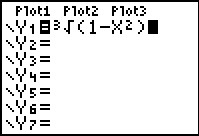
\includegraphics[width=1.9in]{./RelationsandFunctionsGraphics/Equation01.jpg} & 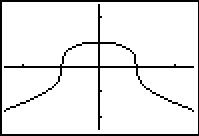
\includegraphics[width=1.9in]{./RelationsandFunctionsGraphics/Equation02.jpg} \\

\end{tabular}

Don't worry if you don't get all of the little bends and curves just right $-$ Calculus is where the art of precise graphing takes center stage.  For now, we will settle with our naive `plug and plot' approach to graphing.  If you feel like all of this tedious computation and plotting is beneath you, then you can reach for a graphing calculator, input the formula as shown above, and graph. \qed

\end{ex}

\medskip

Of all of the points on the graph of an equation, the places where the graph crosses or touches the axes hold special significance.  These are called the \textbf{intercepts} \index{intercept ! definition of} of the graph.  Intercepts come in two distinct varieties: $x$-intercepts and $y$-intercepts.  They are defined below.

\medskip

\colorbox{ResultColor}{\bbm

%\smallskip

\begin{defn}  Suppose the graph of an equation is given.

\label{interceptsdefn}

\begin{itemize}

\item  A point on a graph which is also on the $x$-axis is called an \index{$x$-intercept} \textbf{\boldmath $x$-intercept} of the graph.

\item  A point on a graph which is also on the $y$-axis is called an \index{$y$-intercept} \textbf{\boldmath $y$-intercept} of the graph.

\end{itemize}

\end{defn}

\ebm}

\medskip

In our previous example the graph had two $x$-intercepts, $(-1,0)$ and $(1,0)$, and one $y$-intercept, $(0,1)$.  The graph of an equation can have any number of intercepts, including none at all!  Since $x$-intercepts lie on the $x$-axis, we can find them by setting $y = 0$ in the equation.  Similarly, since $y$-intercepts lie on the $y$-axis, we can find them by setting $x = 0$ in the equation.  Keep in mind, intercepts are \emph{points} and therefore must be written as ordered pairs.  To summarize,

\medskip

\colorbox{ResultColor}{\bbm

%\smallskip

\centerline{\textbf{Finding the Intercepts of the Graph of an Equation}}

\medskip

\hspace{.17in} Given an equation involving $x$ and $y$, we find the intercepts of the graph as follows: \index{intercept ! location of}

\begin{itemize}

\item $x$-intercepts have the form $(x,0)$; set $y = 0$ in the equation and solve for $x$.  

\item $y$-intercepts have the form $(0,y)$; set $x = 0$ in the equation and solve for $y$. 

\end{itemize}

\ebm}

\medskip

Another fact which you may have noticed about the graph in the previous example is that it seems to be symmetric about the $y$-axis.  To actually prove this analytically, we assume $(x,y)$ is a generic point on the graph of the equation. That is, we assume  $x^2 + y^3 = 1$ is true.  As we learned in Section \ref{CartesianPlane},  the point symmetric to $(x,y)$ about the $y$-axis is $(-x,y)$.  To show that the graph is symmetric about the $y$-axis, we need to show that $(-x,y)$ satisfies the equation $x^2 + y^3 = 1$, too.  Substituting $(-x,y)$ into the equation gives

\setlength{\extrarowheight}{2pt}

\[ \begin{array}{rclr}   
(-x)^2+(y)^3 & \stackrel{?}{=} & 1 & \\
   x^2 + y^3 & \stackrel{\checkmark}{=} & 1 & \\ 
   \end{array} \]

Since we are assuming the original equation $x^2 + y^3 = 1$ is true, we have shown that $(-x, y)$ satisfies the equation (since it leads to a true result) and hence is on the graph.  In this way, we can check whether the graph of a given equation possesses any of the symmetries discussed in Section \ref{CartesianPlane}.  We summarize the procedure in the following result.  

\medskip

\colorbox{ResultColor}{\bbm

%\smallskip

\centerline{\textbf{Testing the Graph of an Equation for Symmetry}}
\phantomsection
\label{symmetrytestequations}

\medskip

\hspace{.17in} To test the graph of an equation for symmetry \index{symmetry ! testing an equation for} 

\begin{itemize}

\item about the $y$-axis $\, - \,$ substitute $(-x,y)$ into the equation and simplify. If the result is equivalent to the original equation, the graph is symmetric about the $y$-axis.

\item about the $x$-axis -- substitute $(x,-y)$ into the equation and simplify. If the result is equivalent to the original equation, the graph is symmetric about the $x$-axis.

\item about the origin - substitute $(-x,-y)$ into the equation and simplify. If the result is equivalent to the original equation, the graph is symmetric about the origin.

\end{itemize}

\ebm}

\medskip

Intercepts and symmetry are two tools which can help us sketch the graph of an equation analytically, as demonstrated in the next example.

\begin{ex}  Find the $x$- and $y$-intercepts (if any) of the graph of $(x-2)^2 + y^2 = 1$. Test for symmetry.  Plot additional points as needed to complete the graph.
\label{secondequgraph}

\medskip

{\bf Solution.} To look for $x$-intercepts, we set $y=0$ and solve

\[ \begin{array}{rclr}   

(x-2)^2 + y^2 & = & 1 & \\ 
(x-2)^2 + 0^2 & = & 1 & \\ 
(x-2)^2 & = & 1 & \\
\sqrt{(x-2)^2} & = & \sqrt{1} & \mbox{extract square roots}\\
x - 2 & = & \pm 1 & \\
x  & = & 2 \pm 1 & \\
x  & = & 3, 1 & \\

\end{array} \]

We get two answers for $x$ which correspond to two $x$-intercepts:  $(1,0)$ and $(3,0)$.    Turning our attention to $y$-intercepts, we set $x=0$ and solve

\[ \begin{array}{rclr}   

(x-2)^2 + y^2 & = & 1 & \\ 
(0-2)^2 + y^2 & = & 1 & \\ 
4 + y^2 & = & 1 & \\
y^2 & = & -3 & \\

\end{array} \]

Since there is no real number which squares to a negative number (Do you remember why?), we are forced to conclude that the graph has no $y$-intercepts.

\medskip

Plotting the data we have so far, we get

\begin{center}

\begin{mfpic}[20]{-1}{5}{-2}{2}
\point[3pt]{(1,0), (3,0)}
\footnotesize
\tlabel[cc](1,0.5){$(1,0)$}
\tlabel[cc](3,0.5){$(3,0)$}
\normalsize
\axes
\tlabel[cc](5,-0.5){\scriptsize $x$}
\tlabel[cc](0.5,2){\scriptsize $y$}
\xmarks{1,2,3,4}
\ymarks{-1,1}
\tlpointsep{5pt}
\scriptsize
\axislabels {x}{{$1$} 1, {$2$} 2, {$3$} 3, {$4$} 4}
\axislabels {y}{{$-1$} -1, {$1$} 1}
\normalsize
\end{mfpic}

\end{center}

Moving along to symmetry, we can immediately dismiss the possibility that the graph is symmetric about the $y$-axis or the origin.  If the graph possessed either of these symmetries, then the fact that $(1,0)$ is on the graph would mean $(-1,0)$ would have to be on the graph. (Why?)  Since $(-1,0)$ would be another $x$-intercept (and we've found all of these), the graph can't have $y$-axis or origin symmetry.  The only symmetry left to test is symmetry about the $x$-axis.   To that end, we substitute $(x,-y)$ into the equation and simplify

\[ \begin{array}{rclr}   

(x-2)^2 + y^2 & = & 1 & \\ 
(x-2)^2 + (-y)^2 & \stackrel{?}{=} & 1 & \\ 
(x-2)^2 + y^2 & \stackrel{\checkmark}{=} & 1 & \\

\end{array} \]

Since we have obtained our original equation, we know the graph is symmetric about the $x$-axis.  This means we can cut our `plug and plot' time in half:  whatever happens below the $x$-axis is reflected above the $x$-axis, and vice-versa.  Proceeding as we did in the previous example, we obtain

\begin{center}

\begin{mfpic}[20]{-1}{5}{-2}{2}
\point[3pt]{(1,0), (3,0)}
\circle{(2,0),1}
\normalsize
\axes
\tlabel[cc](5,-0.5){\scriptsize $x$}
\tlabel[cc](0.5,2){\scriptsize $y$}
\xmarks{1,2,3,4}
\ymarks{-1,1}
\tlpointsep{5pt}
\scriptsize
\axislabels {x}{{$1$} 1, {$2$} 2, {$3$} 3, {$4$} 4}
\axislabels {y}{{$-1$} -1, {$1$} 1}
\normalsize
\end{mfpic}
\end{center}

\qed

\end{ex}

A couple of remarks are in order.  First, it is entirely possible to choose a value for $x$ which does not correspond to a point on the graph.  For example, in the previous example, if we solve for $y$ as is our custom, we get
\[y = \pm \sqrt{1-(x-2)^2}.\]
Upon substituting $x=0$ into the equation, we would obtain
\[y = \pm \sqrt{1 - (0-2)^2} = \pm \sqrt{1 - 4} = \pm \sqrt{-3},\]
which is not a real number.  This means there are no points on the graph with an $x$-coordinate of $0$.  When this happens, we move on and try another point.  This is another drawback of the `plug-and-plot' approach to graphing equations.  Luckily, we will devote much of the remainder of this book to developing techniques which allow us to graph entire families of equations quickly.\footnote{Without the use of a calculator, if you can believe it!}  Second, it is instructive to show what would have happened had we tested the equation in the last example for symmetry about the $y$-axis.  Substituting $(-x,y)$ into the equation yields

\[ \begin{array}{rclr}  

(x-2)^2 + y^2 & = & 1 & \\
(-x-2)^2 + y^2 & \stackrel{?}{=} & 1 & \\
((-1)(x+2))^2 + y^2 & \stackrel{?}{=} & 1 & \\
(x+2)^2 + y^2 & \stackrel{?}{=} & 1. & \\

\end{array} \]

This last equation does not \emph{appear} to be equivalent to our original equation.  However, to actually prove that the graph is not symmetric about the $y$-axis, we need to find a point $(x,y)$ on the graph whose reflection $(-x,y)$ is not. Our $x$-intercept $(1,0)$ fits this bill nicely, since if we substitute $(-1,0)$ into the equation we get

\[ \begin{array}{rclr}   

(x-2)^2+y^2 & \stackrel{?}{=} & 1 & \\
(-1-2)^2 + 0^2 & \neq & 1 & \\
9 & \neq & 1. & 

\end{array} \]

This proves that $(-1,0)$ is not on the graph.

\newpage

\subsection{Exercises}

In Exercises \ref{relationfirst} - \ref{relationlast}, graph the given relation.

\begin{enumerate}

\item \{$(-3, 9)$, $\;(-2, 4)$, $\;(-1, 1)$, $\;(0, 0)$, $\;(1, 1)$, $\;(2, 4)$, $\;(3, 9)\}$ \label{relationfirst}
\item \{$(-2, 0)$, $\;(-1, 1)$, $\;(-1, -1)$, $\;(0, 2)$, $\;(0, -2)$, $\;(1, 3)$, $\;(1, -3)\}$

\setcounter{HW}{\value{enumi}}
\end{enumerate}


\begin{multicols}{2}
\begin{enumerate}
\setcounter{enumi}{\value{HW}}

\item  $\left\{ \left(m, 2m \right) \, | \, m = 0, \pm 1, \pm 2 \right\}$
\item  $\left\{ \left(\frac{6}{k}, k \right) \, | \, k = \pm 1, \pm 2, \pm 3, \pm 4, \pm 5, \pm 6 \right\}$

\setcounter{HW}{\value{enumi}}
\end{enumerate}
\end{multicols}


\begin{multicols}{2}
\begin{enumerate}
\setcounter{enumi}{\value{HW}}

\item  $\left\{ \left(n, 4 - n^2\right) \, | \, n = 0, \pm 1, \pm 2 \right\}$
\item  $\left\{ \left(\sqrt{j}, j \right) \, | \, j = 0, 1, 4, 9 \right\}$

\setcounter{HW}{\value{enumi}}
\end{enumerate}
\end{multicols}


\begin{multicols}{2}
\begin{enumerate}
\setcounter{enumi}{\value{HW}}

\item  $\left\{ \left(x, -2 \right) \, | \, x > -4 \right\}$
\item  $\left\{ \left(x, 3 \right) \, | \, x \leq 4 \right\}$

\setcounter{HW}{\value{enumi}}
\end{enumerate}
\end{multicols}

\begin{multicols}{2}
\begin{enumerate}
\setcounter{enumi}{\value{HW}}

\item  $\left\{ \left(-1, y \right) \, | \, y > 1 \right\}$
\item  $\left\{ \left(2, y \right) \, | \, y \leq 5 \right\}$

\setcounter{HW}{\value{enumi}}
\end{enumerate}
\end{multicols}

\begin{multicols}{2}
\begin{enumerate}
\setcounter{enumi}{\value{HW}}

\item $\{ (-2, y) \, | \, -3 < y \leq 4\}$
\item  $\left\{ \left(3,y \right) \, | \, -4 \leq y < 3 \right\}$

\setcounter{HW}{\value{enumi}}
\end{enumerate}
\end{multicols}

\begin{multicols}{2}
\begin{enumerate}
\setcounter{enumi}{\value{HW}}

\item $\{ (x, 2) \, | \, -2 \leq x < 3 \}$
\item  $\left\{ \left(x,-3 \right) \, | \, -4 < x \leq 4 \right\}$

\setcounter{HW}{\value{enumi}}
\end{enumerate}
\end{multicols}

\begin{multicols}{2}
\begin{enumerate}
\setcounter{enumi}{\value{HW}}

\item $\{ (x, y) \, | \, x > -2 \}$
\item  $\left\{ \left(x,y \right) \, | \, x \leq 3 \right\}$

\setcounter{HW}{\value{enumi}}
\end{enumerate}
\end{multicols}

\begin{multicols}{2}
\begin{enumerate}
\setcounter{enumi}{\value{HW}}

\item  $\left\{ \left(x,y \right) \, | \, y < 4 \right\}$
\item  $\left\{ \left(x,y \right) \, | \, x \leq 3, \, y < 2 \right\}$

\setcounter{HW}{\value{enumi}}
\end{enumerate}
\end{multicols}

\begin{multicols}{2}
\begin{enumerate}
\setcounter{enumi}{\value{HW}}

\item  $\left\{ \left(x,y \right) \, | \, x > 0, \, y < 4 \right\}$
\item $\{ (x, y) \, | \, -\sqrt{2} \leq x \leq \frac{2}{3}, \; \pi < y \leq \frac{9}{2} \}$ \label{relationlast}

\setcounter{HW}{\value{enumi}}
\end{enumerate}
\end{multicols}


In Exercises \ref{relationsetfirst} - \ref{relationsetlast}, describe the given relation using either the roster or set-builder method.


\begin{multicols}{2}
\begin{enumerate}
\setcounter{enumi}{\value{HW}}


\item $~$ \label{relationsetfirst}

\begin{mfpic}[15]{-5}{2}{-2}{5}
\point[4pt]{(-4, -1),  (-2, 1),  (0, 3), (1, 4)}
\axes
\tlabel[cc](2,-0.5){\scriptsize $x$}
\tlabel[cc](0.5,5){\scriptsize $y$}
\xmarks{-4,-3,-2,-1,1}
\ymarks{-1,1,2,3,4}
\tlpointsep{5pt}
\scriptsize
\axislabels {x}{{$-4 \hspace{7pt}$} -4, {$-3 \hspace{7pt}$} -3, {$-2 \hspace{7pt}$} -2, {$-1 \hspace{7pt}$} -1, {$1$} 1}
\axislabels {y}{{$-1$} -1, {$1$} 1, {$2$} 2, {$3$} 3, {$4$} 4}
\normalsize
\tcaption{Relation $A$}
\end{mfpic}


\vfill
\columnbreak



\item $~$

\begin{mfpic}[15]{-5}{5}{-1}{4}
\arrow \polyline{(-3,3), (5,3)}
\point[3pt]{(-3,3)}
\axes
\tlabel[cc](5,-0.5){\scriptsize $x$}
\tlabel[cc](0.5,4){\scriptsize $y$}
\xmarks{-4,-3,-2,-1,1,2,3,4}
\ymarks{1,2,3}
\tlpointsep{5pt}
\scriptsize
\axislabels {x}{{$-1 \hspace{7pt}$} -1, {$-2 \hspace{7pt}$} -2, {$-3 \hspace{7pt}$} -3, {$-4 \hspace{7pt}$} -4, {$1$} 1, {$2$} 2, {$3$} 3, {$4$} 4}
\axislabels {y}{{$1$} 1, {$2$} 2, {$3$} 3}
\normalsize
\tcaption{Relation $B$}
\end{mfpic} 


\setcounter{HW}{\value{enumi}}
\end{enumerate}
\end{multicols}


\pagebreak

\begin{multicols}{2}
\begin{enumerate}
\setcounter{enumi}{\value{HW}}

\item $~$

\begin{mfpic}[15]{-1}{4}{-4}{6}
\arrow \polyline{(2,-3), (2,5)}
\pointfillfalse
\point[3pt]{(2,-3)}
\axes
\tlabel[cc](4,-0.5){\scriptsize $x$}
\tlabel[cc](0.5,6){\scriptsize $y$}
\xmarks{1,2,3}
\ymarks{-3,-2,-1,1,2,3,4,5}
\tlpointsep{5pt}
\scriptsize
\axislabels {x}{{$1$} 1, {$2$} 2, {$3$} 3}
\axislabels {y}{ {$-3$} -3,{$-2$} -2, {$-1$} -1, {$1$} 1, {$2$} 2, {$3$} 3, {$4$} 4, {$5$} 5}
\normalsize
\tcaption{Relation $C$}
\end{mfpic} 

\vfill
\columnbreak

\item $~$ 


\begin{mfpic}[15]{-4}{1}{-5}{4}
\polyline{(-2,-4), (-2,3)}
\point[3pt]{(-2,-4)}
\pointfillfalse
\point[3pt]{(-2,3)}
\axes
\tlabel[cc](1,-0.5){\scriptsize $x$}
\tlabel[cc](0.5,4){\scriptsize $y$}
\xmarks{-3,-2,-1}
\ymarks{-4,-3,-2,-1,1,2,3}
\tlpointsep{5pt}
\scriptsize
\axislabels {x}{{$-3 \hspace{7pt}$} -3, {$-2 \hspace{7pt}$} -2, {$-1 \hspace{7pt}$} -1}
\axislabels {y}{{$-4$} -4,{$-3$} -3, {$-2$} -2, {$-1$} -1, {$1$} 1, {$2$} 2, {$3$} 3}
\normalsize
\tcaption{Relation $D$}
\end{mfpic}

\setcounter{HW}{\value{enumi}}
\end{enumerate}
\end{multicols}

\begin{multicols}{2}
\begin{enumerate}
\setcounter{enumi}{\value{HW}}

\item $~$

\begin{mfpic}[15]{-5}{5}{-1}{4}
\polyline{(-4,2), (3,2)}
\point[3pt]{(-4,2)}
\pointfillfalse
\point[3pt]{(3,2)}
\axes
\tlabel[cc](5,-0.5){\scriptsize $x$}
\tlabel[cc](0.5,4){\scriptsize $y$}
\xmarks{-4,-3,-2,-1,1,2,3,4}
\ymarks{1,2,3}
\tlpointsep{5pt}
\scriptsize
\axislabels {x}{{$-4 \hspace{7pt}$} -4,{$-3 \hspace{7pt}$} -3, {$-2 \hspace{7pt}$} -2, {$-1 \hspace{7pt}$} -1, {$1$} 1, {$2$} 2, {$3$} 3, {$4$} 4}
\axislabels {y}{{$1$} 1, {$2$} 2, {$3$} 3}
\normalsize
\tcaption{Relation $E$}
\end{mfpic}

\vfill
\columnbreak

\item $~$

\begin{mfpic}[15]{-4}{4}{-1}{5}
\fillcolor[gray]{.7}
\gfill \rect{(-4,0), (3.75,4.75)}
\axes
\tlabel[cc](4,-0.5){\scriptsize $x$}
\tlabel[cc](0.5,5){\scriptsize $y$}
\xmarks{-3,-2,-1,1,2,3}
\ymarks{1,2,3,4}
\tlpointsep{5pt}
\scriptsize
\axislabels {x}{{$-3 \hspace{7pt}$} -3,{$-2 \hspace{7pt}$} -2, {$-1 \hspace{7pt}$} -1, {$1$} 1, {$2$} 2, {$3$} 3}
\axislabels {y}{ {$1$} 1, {$2$} 2, {$3$} 3, , {$4$} 4}
\normalsize
\tcaption{Relation $F$}
\end{mfpic} 

\setcounter{HW}{\value{enumi}}
\end{enumerate}
\end{multicols}

\begin{multicols}{2}
\begin{enumerate}
\setcounter{enumi}{\value{HW}}

\item $~$

\begin{mfpic}[15]{-4}{4}{-4}{4}
\fillcolor[gray]{.7}
\gfill \rect{(-1.97,-3.75), (3.75,3.75)}
\arrow \reverse \arrow \dashed \polyline{(-2,-4), (-2,4)}
\axes
\tlabel[cc](4,-0.5){\scriptsize $x$}
\tlabel[cc](0.5,4){\scriptsize $y$}
\xmarks{-3,-2,-1,1,2,3}
\ymarks{-3,-2,-1,1,2,3}
\tlpointsep{5pt}
\scriptsize
\axislabels {x}{{$-3 \hspace{7pt}$} -3,{$-2 \hspace{7pt}$} -2,{$-1 \hspace{7pt}$} -1,{$1$} 1,{$2$} 2,{$3$} 3}
\axislabels {y}{ {$-3$} -3,{$-2$} -2, {$-1$} -1, {$1$} 1, {$2$} 2, {$3$} 3}
\normalsize
\tcaption{Relation $G$}
\end{mfpic} 


\vfill
\columnbreak

\item $~$

\begin{mfpic}[15]{-4.5}{4}{-4}{4}

\fillcolor[gray]{.7}
\gfill \rect{(-2.97,-3.75), (1.97,3.75)}
\arrow \reverse \arrow \dashed \polyline{(-3,-4), (-3,4)}
\arrow \reverse \arrow \polyline{(2,-4), (2,4)}
\axes
\tlabel[cc](4,-0.5){\scriptsize $x$}
\tlabel[cc](0.5,4){\scriptsize $y$}
\xmarks{-4,-3,-2,-1,1,2,3}
\ymarks{-3,-2,-1,1,2,3}
\tlpointsep{5pt}
\scriptsize
\axislabels {x}{{$-4 \hspace{7pt}$} -4,{$-3 \hspace{7pt}$} -3,{$-2 \hspace{7pt}$} -2,{$-1 \hspace{7pt}$} -1,{$1$} 1,{$2$} 2,{$3$} 3}
\axislabels {y}{ {$-3$} -3,{$-2$} -2, {$-1$} -1, {$1$} 1, {$2$} 2, {$3$} 3}
\normalsize
\tcaption{Relation $H$}
\end{mfpic}


\setcounter{HW}{\value{enumi}}
\end{enumerate}
\end{multicols}


\pagebreak

\begin{multicols}{2}
\begin{enumerate}
\setcounter{enumi}{\value{HW}}

\item $~$

\begin{mfpic}[15]{-1.5}{6}{-1.5}{6}
\fillcolor[gray]{.7}
\gfill \rect{(0,0), (5.75,5.75)}
\axes
\tlabel[cc](6,-0.5){\scriptsize $x$}
\tlabel[cc](0.5,6){\scriptsize $y$}
\xmarks{-1,1,2,3,4,5}
\ymarks{-1,1,2,3,4,5}
\tlpointsep{5pt}
\scriptsize
\axislabels {x}{ {$-1 \hspace{7pt}$} -1, {$1$} 1, {$2$} 2, {$3$} 3, {$4$} 4, {$5$} 5}
\axislabels {y}{ {$-1$} -1, {$1$} 1, {$2$} 2, {$3$} 3, {$4$} 4, {$5$} 5}
\normalsize
\tcaption{Relation $I$}
\end{mfpic} 

\vfill
\columnbreak

\item $~$ \label{relationsetlast}

\begin{mfpic}[15]{-4.5}{5.5}{-4}{3}
\fillcolor[gray]{.7}
\gfill \rect{(-3.97, -2.97), (4.97, 1.97)}
\dashed \polyline{(-4, -3), (-4, 2)}
\dashed \polyline{(-4, 2), (5, 2)}
\dashed \polyline{(5, 2), (5, -3)}
\dashed \polyline{(5, -3), (-4, -3)}
\axes
\tlabel[cc](5.5,-0.5){\scriptsize $x$}
\tlabel[cc](0.5,3){\scriptsize $y$}
\xmarks{-4,-3,-2,-1,1,2,3,4,5}
\ymarks{-3,-2,-1,1,2}
\tlpointsep{5pt}
\scriptsize
\axislabels {x}{{$-4 \hspace{7pt}$} -4, {$-3 \hspace{7pt}$} -3, {$-2 \hspace{7pt}$} -2, {$-1 \hspace{7pt}$} -1, {$1$} 1, {$2$} 2, {$3$} 3, {$4$} 4, {$5$} 5}
\axislabels {y}{{$-3$} -3, {$-2$} -2, {$-1$} -1, {$1$} 1, {$2$} 2}
\normalsize
\tcaption{Relation $J$}
\end{mfpic}


\setcounter{HW}{\value{enumi}}
\end{enumerate}
\end{multicols}


In Exercises \ref{graphlinefirst} - \ref{graphlinelast}, graph the given line.

\begin{multicols}{2}
\begin{enumerate}
\setcounter{enumi}{\value{HW}}

\item $x = -2$ \label{graphlinefirst}
\item $x = 3$

\setcounter{HW}{\value{enumi}}
\end{enumerate}
\end{multicols}

\begin{multicols}{2}
\begin{enumerate}
\setcounter{enumi}{\value{HW}}

\item $y = 3$
\item $y = -2$

\setcounter{HW}{\value{enumi}}
\end{enumerate}
\end{multicols}



\begin{multicols}{2}
\begin{enumerate}
\setcounter{enumi}{\value{HW}}

\item  $x=0$
\item $y=0$ \label{graphlinelast}

\setcounter{HW}{\value{enumi}}
\end{enumerate}
\end{multicols}


Some relations are fairly easy to describe in words or with the roster method but are rather difficult, if not impossible, to graph. Discuss with your classmates how you might graph the relations given in Exercises \ref{cannotgraphfirst} - \ref{cannotgraphlast}.  Please note that in the notation below we are using the \index{ellipsis (\ldots)} ellipsis, \ldots, to denote that the list does not end, but rather, continues to follow the established pattern indefinitely.  For the relations in Exercises \ref{cannotgraphfirst} and \ref{cannotgraphsecond}, give two examples of points which belong to the relation and two points which do not belong to the relation.


\begin{enumerate}
\setcounter{enumi}{\value{HW}}


\item $\{(x, y) \, | \, x \mbox{ is an odd integer, and } y \mbox{ is an even integer.}\}$ \label{cannotgraphfirst}
\item $\{(x, 1) \, | \, x \mbox{ is an irrational number }\}$ \label{cannotgraphsecond}
\item $\{(1, 0), (2, 1), (4, 2), (8, 3), (16, 4), (32, 5), \ldots \}$
\item $\{\ldots, (-3, 9), (-2, 4), (-1, 1), (0, 0), (1, 1), (2, 4), (3, 9), \ldots \}$ \label{cannotgraphlast}

\setcounter{HW}{\value{enumi}}
\end{enumerate}


For each equation given in Exercises \ref{oldonethreefirst} - \ref{oldonethreelast}:

\begin{itemize}

\item Find the $x$- and $y$-intercept(s) of the graph, if any exist.

\item Follow the procedure in Example \hspace{-.1in} ~\ref{firstequgraph} to create a table of sample points on the graph of the equation.

\item Plot the sample points and create a rough sketch of the graph of the equation.

\item Test for symmetry.  If the equation appears to fail any of the symmetry tests, find a point on the graph of the equation whose reflection fails to be on the graph as was done at the end of Example \ref{secondequgraph}

\end{itemize}

\begin{multicols}{2}
\begin{enumerate}
\setcounter{enumi}{\value{HW}}



\item $y = x^{2} + 1$ \label{oldonethreefirst}
\item  $y = x^2-2x-8$

\setcounter{HW}{\value{enumi}}
\end{enumerate}
\end{multicols}

\begin{multicols}{2}
\begin{enumerate}
\setcounter{enumi}{\value{HW}}

\item $y = x^{3} - x$
\item  $y = \frac{x^3}{4} - 3x$

\setcounter{HW}{\value{enumi}}
\end{enumerate}
\end{multicols}

\begin{multicols}{2}
\begin{enumerate}
\setcounter{enumi}{\value{HW}}

\item $y = \sqrt{x - 2}$
\item  $y = 2 \sqrt{x+4} - 2$

\setcounter{HW}{\value{enumi}}
\end{enumerate}
\end{multicols}

\begin{multicols}{2}
\begin{enumerate}
\setcounter{enumi}{\value{HW}}

\item $3x - y = 7$
\item  $3x-2y = 10$

\setcounter{HW}{\value{enumi}}
\end{enumerate}
\end{multicols}

\begin{multicols}{2}
\begin{enumerate}
\setcounter{enumi}{\value{HW}}

\item  $(x+2)^2+y^2 = 16$

\item $x^{2} - y^{2} = 1$

\setcounter{HW}{\value{enumi}}
\end{enumerate}
\end{multicols}

\begin{multicols}{2}
\begin{enumerate}
\setcounter{enumi}{\value{HW}}

\item  $4y^2 - 9x^2 = 36$
\item $x^{3}y = -4$ \label{oldonethreelast}

\setcounter{HW}{\value{enumi}}
\end{enumerate}
\end{multicols}

The procedures which we have outlined in the Examples of this section and used in Exercises \ref{oldonethreefirst} -  \ref{oldonethreelast} all rely on the fact that the equations were ``well-behaved''.  Not everything in Mathematics is quite so tame, as the following equations will show you.  Discuss with your classmates how you might approach graphing the equations given in Exercises \ref{listofcurvesfirst} - \ref{listofcurveslast}.  What difficulties arise when trying to apply the various tests and procedures given in this section?  For more information, including pictures of the curves, each curve name is a link to its page at www.wikipedia.org.  For a much longer list of fascinating curves, click \href{http://en.wikipedia.org/wiki/List_of_curves}{\underline{here}}.


\begin{multicols}{2}
\begin{enumerate}
\setcounter{enumi}{\value{HW}}

\item \label{listofcurvesfirst} $x^{3} + y^{3} - 3xy = 0\;$ \href{http://en.wikipedia.org/wiki/Folium_of_descartes}{\underline{Folium of Descartes}}
\item $x^{4} = x^{2} + y^{2}\;$ \href{http://en.wikipedia.org/wiki/Kampyle_of_Eudoxus}{\underline{Kampyle of Eudoxus}}
\setcounter{HW}{\value{enumi}}
\end{enumerate}
\end{multicols}

\begin{multicols}{2}
\begin{enumerate}
\setcounter{enumi}{\value{HW}}


\item $y^{2} = x^{3} + 3x^{2}\;$ \href{http://en.wikipedia.org/wiki/Tschirnhausen_cubic}{\underline{Tschirnhausen cubic}}
\item \label{listofcurveslast} $(x^{2} + y^{2})^{2} = x^{3} + y^{3}\;$ \href{http://en.wikipedia.org/wiki/Crooked_egg_curve}{\underline{Crooked egg}} 

\setcounter{HW}{\value{enumi}}
\end{enumerate}
\end{multicols}

\begin{enumerate}
\setcounter{enumi}{\value{HW}}

\item  With the help of your classmates, find examples of equations whose graphs possess 

\begin{itemize}

\item  symmetry about the $x$-axis only

\item  symmetry about the $y$-axis only

\item  symmetry about the origin only

\item  symmetry about the $x$-axis, $y$-axis, and origin

\end{itemize}

Can you find an example of an equation whose graph possesses exactly \textit{two} of the symmetries listed above?  Why or why not?

\end{enumerate}

\newpage

\subsection{Answers}

\begin{multicols}{2}
\begin{enumerate}

\item $~$ 

\begin{mfpic}[13]{-4}{4}{-1}{10}
\point[4pt]{(-3, 9), (-2, 4), (-1, 1), (0, 0), (1, 1), (2, 4), (3, 9)}
\axes
\tlabel[cc](4,-0.5){\scriptsize $x$}
\tlabel[cc](0.5,10){\scriptsize $y$}
\xmarks{-3,-2,-1,1,2,3}
\ymarks{1,2,3,4,5,6,7,8,9}
\tlpointsep{5pt}
\scriptsize
\axislabels {x}{{$-3 \hspace{7pt}$} -3, {$-2 \hspace{7pt}$} -2, {$-1 \hspace{7pt}$} -1, {$1$} 1, {$2$} 2, {$3$} 3}
\axislabels {y}{{$1$} 1, {$2$} 2, {$3$} 3, {$4$} 4, {$5$} 5, {$6$} 6, {$7$} 7, {$8$} 8, {$9$} 9}
\normalsize
\end{mfpic}


\vfill
\columnbreak

\item $~$ 

\begin{mfpic}[15]{-3}{3}{-4}{4}
\point[4pt]{(-2, 0), (-1, -1), (-1,1), (0,2), (0,-2), (1,3), (1,-3)}
\axes
\tlabel[cc](3,-0.5){\scriptsize $x$}
\tlabel[cc](0.5,4){\scriptsize $y$}
\xmarks{-2,-1,1,2}
\ymarks{-3,-2,-1,1,2,3}
\tlpointsep{5pt}
\scriptsize
\axislabels {x}{{$-2 \hspace{7pt}$} -2, {$-1 \hspace{7pt}$} -1, {$1$} 1, {$2$} 2}
\axislabels {y}{{$-3$} -3, {$-2$} -2, {$-1$} -1, {$1$} 1, {$2$} 2, {$3$} 3}
\normalsize
\end{mfpic}

\setcounter{HW}{\value{enumi}}
\end{enumerate}
\end{multicols}

\begin{multicols}{2}
\begin{enumerate}
\setcounter{enumi}{\value{HW}}

\item $~$

\begin{mfpic}[15]{-3}{3}{-5}{5}
\point[4pt]{(-2, -4), (-1, -2), (0, 0), (1, 2), (2,4)}
\axes
\tlabel[cc](3,-0.5){\scriptsize $x$}
\tlabel[cc](0.5,5){\scriptsize $y$}
\xmarks{-2,-1,1,2}
\ymarks{-4,-3,-2,-1,1,2,3,4}
\tlpointsep{5pt}
\scriptsize
\axislabels {x}{{$-2 \hspace{7pt}$} -2, {$-1 \hspace{7pt}$} -1, {$1$} 1, {$2$} 2}
\axislabels {y}{  {$-1$} -1, {$-2$} -2, {$-3$} -3, {$-4$} -4, {$1$} 1, {$2$} 2, {$3$} 3, {$4$} 4}
\normalsize
\end{mfpic} 

\vfill
\columnbreak

\item $~$

\begin{mfpic}[12]{-7}{7}{-7}{7}
\point[4pt]{(6, 1), (-6, -1), (3, 2), (-3, -2), (2,3), (-2, -3), (-1.5,-4), (1.5,4), (-1.2,-5), (1.2,5), (-1,-6), (1,6) }
\axes
\tlabel[cc](7,-0.5){\scriptsize $x$}
\tlabel[cc](0.5,7){\scriptsize $y$}
\xmarks{-6,-5,-4,-3,-2,-1,1,2,3,4,5,6}
\ymarks{-6,-5,-4,-3,-2,-1,1,2,3,4,5,6}
\tlpointsep{5pt}
\scriptsize
\axislabels {x}{{$-6 \hspace{7pt}$} -6, {$-5 \hspace{7pt}$} -5, {$-4 \hspace{7pt}$} -4, {$-3 \hspace{7pt}$} -3, {$-2 \hspace{7pt}$} -2, {$-1 \hspace{7pt}$} -1, {$1$} 1, {$2$} 2, {$3$} 3, {$4$} 4, {$5$} 5, {$6$} 6}
\axislabels {y}{{$-6$} -6, {$-5$} -5,{$-4$} -4, {$-3$} -3,{$-2$} -2, {$-1$} -1, {$1$} 1, {$2$} 2, {$3$} 3, {$4$} 4, {$5$} 5, {$6$} 6}
\normalsize
\end{mfpic} 




\setcounter{HW}{\value{enumi}}
\end{enumerate}
\end{multicols}

\begin{multicols}{2}
\begin{enumerate}
\setcounter{enumi}{\value{HW}}

\item $~$

\begin{mfpic}[15]{-3}{3}{-1}{5}
\point[4pt]{(0, 4), (1, 3), (-1, 3), (2, 0), (-2,0)}
\axes
\tlabel[cc](3,-0.5){\scriptsize $x$}
\tlabel[cc](0.5,5){\scriptsize $y$}
\xmarks{-2,-1,1,2}
\ymarks{1,2,3,4}
\tlpointsep{5pt}
\scriptsize
\axislabels {x}{{$-2 \hspace{7pt}$} -2, {$-1 \hspace{7pt}$} -1, {$1$} 1, {$2$} 2}
\axislabels {y}{ {$1$} 1, {$2$} 2, {$3$} 3, {$4$} 4}
\normalsize
\end{mfpic} 

\vfill
\columnbreak

\item $~$

\begin{mfpic}[10]{-1}{4}{-1}{10}
\point[4pt]{(0,0), (1,1), (2,4), (3,9)}
\axes
\tlabel[cc](4,-0.5){\scriptsize $x$}
\tlabel[cc](0.5,10){\scriptsize $y$}
\xmarks{1,2,3}
\ymarks{1,2,3,4,5,6,7,8,9}
\tlpointsep{5pt}
\scriptsize
\axislabels {x}{{$1$} 1, {$2$} 2, {$3$} 3}
\axislabels {y}{{$1$} 1, {$2$} 2, {$3$} 3, {$4$} 4, {$5$} 5, {$6$} 6, {$7$} 7, {$8$} 8, {$9$} 9}
\normalsize
\end{mfpic} 

\setcounter{HW}{\value{enumi}}
\end{enumerate}
\end{multicols}

\pagebreak

\begin{multicols}{2}
\begin{enumerate}
\setcounter{enumi}{\value{HW}}

\item $~$

\begin{mfpic}[15]{-5}{5}{-4}{1}
\arrow \polyline{(-4,-2), (5,-2)}
\gclear \circle{(-4,-2),0.1}
\circle{(-4,-2),0.1}
\axes
\xmarks{-4,-3,-2,-1,1,2,3,4}
\ymarks{-3,-2,-1}
\tlpointsep{5pt}
\scriptsize
\tlabel[cc](5,-0.5){\scriptsize $x$}
\tlabel[cc](0.5,1){\scriptsize $y$}
\axislabels {x}{{$-4 \hspace{7pt}$} -4, {$-3 \hspace{7pt}$} -3,{$-2 \hspace{7pt}$} -2, {$-1 \hspace{7pt}$} -1, {$1$} 1, {$2$} 2, {$3$} 3, {$4$} 4}
\axislabels {y}{ {$-3$} -3,  {$-1$} -1,}
\normalsize
\end{mfpic} 

\vfill
\columnbreak

\item $~$ 

\begin{mfpic}[15]{-5}{5}{-1}{4}
\arrow \polyline{(4,3), (-5,3)}
\point[3pt]{(4,3)}
\axes
\tlabel[cc](5,-0.5){\scriptsize $x$}
\tlabel[cc](0.5,4){\scriptsize $y$}
\xmarks{-4,-3,-2,-1,1,2,3,4}
\ymarks{1,2,3}
\tlpointsep{5pt}
\scriptsize
\axislabels {x}{{$-1 \hspace{7pt}$} -1, {$-2 \hspace{7pt}$} -2, {$-3 \hspace{7pt}$} -3, {$-4 \hspace{7pt}$} -4, {$1$} 1, {$2$} 2, {$3$} 3, {$4$} 4}
\axislabels {y}{{$1$} 1, {$2$} 2, {$3$} 3}
\normalsize
\end{mfpic} 

\setcounter{HW}{\value{enumi}}
\end{enumerate}
\end{multicols}

\begin{multicols}{2}
\begin{enumerate}
\setcounter{enumi}{\value{HW}}

\item $~$

\begin{mfpic}[15]{-2}{3}{-1}{9}
\arrow \polyline{(-1,1), (-1,9)}
\pointfillfalse
\point[3pt]{(-1,1)}
\axes
\xmarks{-1,1,2}
\ymarks{1,2,3,4,5,6,7,8}
\tlpointsep{5pt}
\scriptsize
\tlabel[cc](3,-0.5){\scriptsize $x$}
\tlabel[cc](0.5,9){\scriptsize $y$}
\axislabels {x}{{$-1 \hspace{7pt}$} -1, {$1$} 1, {$2$} 2}
\axislabels {y}{{$1$} 1, {$2$} 2, {$3$} 3, {$4$} 4, {$5$} 5, {$6$} 6, {$7$} 7, {$8$} 8}
\normalsize
\end{mfpic} 

\vfill
\columnbreak

\item $~$ 

\begin{mfpic}[15]{-1}{4}{-4}{6}
\arrow \polyline{(2,5), (2,-4)}
\point[3pt]{(2,5)}
\axes
\tlabel[cc](4,-0.5){\scriptsize $x$}
\tlabel[cc](0.5,6){\scriptsize $y$}
\xmarks{1,2,3}
\ymarks{-3,-2,-1,1,2,3,4,5}
\tlpointsep{5pt}
\scriptsize
\axislabels {x}{{$1$} 1, {$2$} 2, {$3$} 3}
\axislabels {y}{ {$-3$} -3,{$-2$} -2, {$-1$} -1, {$1$} 1, {$2$} 2, {$3$} 3, {$4$} 4, {$5$} 5}
\normalsize
\end{mfpic} 

\setcounter{HW}{\value{enumi}}
\end{enumerate}
\end{multicols}

\begin{multicols}{2}
\begin{enumerate}
\setcounter{enumi}{\value{HW}}


\item $~$

\begin{mfpic}[15]{-4}{1}{-4}{5}
\polyline{(-2,-3), (-2,4)}
\point[3pt]{(-2,4)}
\pointfillfalse
\point[3pt]{(-2,-3)}
\axes
\tlabel[cc](1,-0.5){\scriptsize $x$}
\tlabel[cc](0.5,5){\scriptsize $y$}
\xmarks{-3,-2,-1}
\ymarks{-3,-2,-1,1,2,3,4}
\tlpointsep{5pt}
\scriptsize
\axislabels {x}{{$-3 \hspace{7pt}$} -3, {$-2 \hspace{7pt}$} -2, {$-1 \hspace{7pt}$} -1}
\axislabels {y}{{$-3$} -3, {$-2$} -2, {$-1$} -1, {$1$} 1, {$2$} 2, {$3$} 3, {$4$} 4}
\normalsize
\end{mfpic}

\vfill
\columnbreak

\item $~$


\begin{mfpic}[15]{-1}{4}{-5}{4}
\polyline{(3,-4), (3,3)}
\point[3pt]{(3,-4)}
\pointfillfalse
\point[3pt]{(3,3)}
\axes
\tlabel[cc](4,-0.5){\scriptsize $x$}
\tlabel[cc](0.5,4){\scriptsize $y$}
\xmarks{1,2,3}
\ymarks{-4,-3,-2,-1,1,2,3}
\tlpointsep{5pt}
\scriptsize
\axislabels {x}{{$1$} 1, {$2$} 2, {$3$} 3}
\axislabels {y}{{$-4$} -4,{$-3$} -3, {$-2$} -2, {$-1$} -1, {$1$} 1, {$2$} 2, {$3$} 3}
\normalsize
\end{mfpic}

\setcounter{HW}{\value{enumi}}
\end{enumerate}
\end{multicols}



\pagebreak


\begin{multicols}{2}
\begin{enumerate}
\setcounter{enumi}{\value{HW}}


\item $~$

\begin{mfpic}[15]{-5}{5}{-1}{4}
\polyline{(-2,2), (3,2)}
\point[3pt]{(-2,2)}
\pointfillfalse
\point[3pt]{(3,2)}
\axes
\tlabel[cc](5,-0.5){\scriptsize $x$}
\tlabel[cc](0.5,4){\scriptsize $y$}
\xmarks{-4,-3,-2,-1,1,2,3,4}
\ymarks{1,2,3}
\tlpointsep{5pt}
\scriptsize
\axislabels {x}{{$-4 \hspace{7pt}$} -4,{$-3 \hspace{7pt}$} -3, {$-2 \hspace{7pt}$} -2, {$-1 \hspace{7pt}$} -1, {$1$} 1, {$2$} 2, {$3$} 3, {$4$} 4}
\axislabels {y}{{$1$} 1, {$2$} 2, {$3$} 3}
\normalsize
\end{mfpic}

\vfill
\columnbreak

\item $~$

\begin{mfpic}[15]{-5}{5}{-4}{1}
\polyline{(-4,-3), (4,-3)}
\point[3pt]{(4,-3)}
\pointfillfalse
\point[3pt]{(-4,-3)}
\axes
\tlabel[cc](5,-0.5){\scriptsize $x$}
\tlabel[cc](0.5,1){\scriptsize $y$}
\xmarks{-4,-3,-2,-1,1,2,3,4}
\ymarks{-1,-2,-3}
\tlpointsep{5pt}
\scriptsize
\axislabels {x}{{$-4 \hspace{7pt}$} -4,{$-3 \hspace{7pt}$} -3, {$-2 \hspace{7pt}$} -2, {$-1 \hspace{7pt}$} -1, {$1$} 1, {$2$} 2, {$3$} 3, {$4$} 4}
\axislabels {y}{{$-1$} -1, {$-2$} -2, {$-3$} -3}
\normalsize
\end{mfpic}

\setcounter{HW}{\value{enumi}}
\end{enumerate}
\end{multicols}



\begin{multicols}{2}
\begin{enumerate}
\setcounter{enumi}{\value{HW}}


\item $~$

\begin{mfpic}[15]{-3}{4}{-4}{4}
\fillcolor[gray]{.7}
\gfill \rect{(-1.97,-3.75), (3.75,3.75)}
\dashed \arrow \reverse \arrow \polyline{(-2,4), (-2,-4)}
\axes
\tlabel[cc](4,-0.5){\scriptsize $x$}
\tlabel[cc](0.5,4){\scriptsize $y$}
\xmarks{-2,-1,1,2,3}
\ymarks{-3,-2,-1,1,2,3}
\tlpointsep{5pt}
\scriptsize
\axislabels {x}{{$3$} 3, {$2$} 2, {$1$} 1, {$-2 \hspace{6pt}$} -2, {$-1 \hspace{6pt}$} -1}
\axislabels {y}{ {$-3$} -3,{$-2$} -2, {$-1$} -1, {$1$} 1, {$2$} 2, {$3$} 3}
\normalsize
\end{mfpic} 


\vfill
\columnbreak

\item $~$

\begin{mfpic}[15]{-1}{4}{-4}{4}
\fillcolor[gray]{.7}
\gfill \rect{(-1,-3.75), (3,3.75)}
\arrow \reverse \arrow \polyline{(3,4), (3,-4)}
\axes
\tlabel[cc](4,-0.5){\scriptsize $x$}
\tlabel[cc](0.5,4){\scriptsize $y$}
\xmarks{1,2,3}
\ymarks{-3,-2,-1,1,2,3}
\tlpointsep{5pt}
\scriptsize
\axislabels {x}{{$1$} 1, {$2$} 2, {$3$} 3}
\axislabels {y}{ {$-3$} -3,{$-2$} -2, {$-1$} -1, {$1$} 1, {$2$} 2, {$3$} 3}
\normalsize
\end{mfpic} 

\setcounter{HW}{\value{enumi}}
\end{enumerate}
\end{multicols}

\begin{multicols}{2}
\begin{enumerate}
\setcounter{enumi}{\value{HW}}


\item $~$

\begin{mfpic}[15]{-4}{4}{-1}{5}

\fillcolor[gray]{.7}
\gfill \rect{(-3.75,-1), (3.75,3.97)}
\arrow \reverse \arrow \dashed \polyline{(-4,4), (4,4)}
\axes
\tlabel[cc](4,-0.5){\scriptsize $x$}
\tlabel[cc](0.5,5){\scriptsize $y$}
\xmarks{-3,-2,-1,1,2,3}
\ymarks{1,2,3,4}
\tlpointsep{5pt}
\scriptsize
\axislabels {x}{{$-3 \hspace{7pt}$} -3,{$-2 \hspace{7pt}$} -2, {$-1 \hspace{7pt}$} -1, {$1$} 1, {$2$} 2, {$3$} 3}
\axislabels {y}{ {$1$} 1, {$2$} 2, {$3$} 3, {$4$} 4}
\normalsize
\end{mfpic} 

\vfill
\columnbreak


\item $~$

\begin{mfpic}[15]{-1}{4}{-4}{4}
\fillcolor[gray]{.7}
\gfill \rect{(-0.75,-3.75), (3,1.97)}
\arrow \polyline{(3,2), (3,-4)}
\arrow \reverse \dashed \polyline{(-1,2), (3,2)}
\pointfillfalse
\point[3pt]{(3,2)}
\axes
\tlabel[cc](4,-0.5){\scriptsize $x$}
\tlabel[cc](0.5,4){\scriptsize $y$}
\xmarks{1,2,3}
\ymarks{-3,-2,-1,1,2,3}
\tlpointsep{5pt}
\scriptsize
\axislabels {x}{{$1$} 1, {$2$} 2, {$3$} 3}
\axislabels {y}{ {$-3$} -3,{$-2$} -2, {$-1$} -1, {$1$} 1, {$2$} 2, {$3$} 3}
\normalsize
\end{mfpic} 

\setcounter{HW}{\value{enumi}}
\end{enumerate}
\end{multicols}

\begin{multicols}{2}
\begin{enumerate}
\setcounter{enumi}{\value{HW}}


\item $~$

\begin{mfpic}[15]{-2}{4}{-1}{5}
\fillcolor[gray]{.7}
\gfill \rect{(0.03,-0.75), (3.75,3.97)}
\arrow  \dashed \polyline{(0,4), (4,4)}
\arrow \dashed \polyline{(0,4), (0,-1)}
\arrow \polyline{(0,4), (0,5)}
\arrow \reverse \arrow \polyline{(-2,0), (4,0)}
\tlabel[cc](4,-0.5){\scriptsize $x$}
\tlabel[cc](0.5,5){\scriptsize $y$}
\xmarks{-1,1,2,3}
\ymarks{1,2,3,4}
\pointfillfalse
\point[3pt]{(0,4)}
\tlpointsep{5pt}
\scriptsize
\axislabels {x}{{$-1 \hspace{7pt}$} -1, {$1$} 1, {$2$} 2, {$3$} 3}
\axislabels {y}{ {$1$} 1, {$2$} 2, {$3$} 3, {$4$} 4}
\normalsize
\end{mfpic} 

\vfill
\columnbreak

\item $~$

\begin{mfpic}[15]{-3}{2}{-1}{6}
\fillcolor[gray]{.7}
\gfill \rect{(-1.38, 3.17), (0.63, 4.47)}
\polyline{(-1.414, 3.1415), (-1.414, 4.5)}
\polyline{(-1.414, 4.5), (0.6667, 4.5)}
\polyline{(0.6667, 4.5), (0.6667, 3.1415)}
\dashed \polyline{(0.6667, 3.1415), (-1.414, 3.1415)}
\pointfillfalse
\point[3pt]{(-1.414, 3.1415), (0.6667, 3.1415)}
\axes
\tlabel[cc](2,-0.5){\scriptsize $x$}
\tlabel[cc](0.5,6){\scriptsize $y$}
\xmarks{-2,-1,1}
\ymarks{1,2,3,4,5}
\tlpointsep{5pt}
\scriptsize
\axislabels {x}{{$-2 \hspace{7pt}$} -2, {$-1 \hspace{7pt}$} -1, {$1$} 1}
\axislabels {y}{{$1$} 1, {$2$} 2, {$3$} 3, {$4$} 4, {$5$} 5}
\normalsize
\end{mfpic}

\setcounter{HW}{\value{enumi}}
\end{enumerate}
\end{multicols}


\begin{multicols}{2}
\begin{enumerate}
\setcounter{enumi}{\value{HW}}

\item $A = \{(-4, -1),  (-2, 1),  (0, 3), (1, 4)\}$

\item $B = \left\{ \left(x,3 \right) \, | \, x \geq -3 \right\}$



\setcounter{HW}{\value{enumi}}
\end{enumerate}
\end{multicols}

\begin{multicols}{2}
\begin{enumerate}
\setcounter{enumi}{\value{HW}}

\item $C = \{ \left(2,y) \, | \, y > -3 \right\}$

\item $D = \{ \left(-2,y) \, | \, -4 \leq y < 3 \right\}$

\setcounter{HW}{\value{enumi}}
\end{enumerate}
\end{multicols}

\begin{multicols}{2}
\begin{enumerate}
\setcounter{enumi}{\value{HW}}

\item $E = \left\{ \left(x,2 \right) \, | \, -4 \leq x < 3 \right\}$
\item $F = \{ \left(x,y) \, | \, y \geq 0 \right\}$

\setcounter{HW}{\value{enumi}}
\end{enumerate}
\end{multicols}

\begin{multicols}{2}
\begin{enumerate}
\setcounter{enumi}{\value{HW}}

\item $G = \left\{ \left(x,y \right) \, | \, x > -2 \right\}$
\item $H = \left\{ \left(x,y \right) \, | \, -3 < x \leq 2 \right\}$

\setcounter{HW}{\value{enumi}}
\end{enumerate}
\end{multicols}

\begin{multicols}{2}
\begin{enumerate}
\setcounter{enumi}{\value{HW}}


\item $I = \{ \left(x,y) \, | \, x \geq 0, \! y \geq 0\right\}$

\item $J = \{(x, y) \, | \, -4 < x < 5, \; -3 < y < 2\}$

\setcounter{HW}{\value{enumi}}
\end{enumerate}
\end{multicols}

\begin{multicols}{2}
\begin{enumerate}
\setcounter{enumi}{\value{HW}}

\item $~$ 

\begin{mfpic}[15]{-4}{1}{-4}{4}
\arrow \reverse \arrow \polyline{(-2,-4), (-2,4)}
\axes
\tlabel[cc](1,-0.5){\scriptsize $x$}
\tlabel[cc](0.5,4){\scriptsize $y$}
\xmarks{-3,-2,-1}
\ymarks{1,2,3,-1,-2,-3}
\tlpointsep{5pt}
\scriptsize
\axislabels {x}{{$-3 \hspace{7pt}$} -3, {$-2 \hspace{7pt}$} -2, {$-1 \hspace{7pt}$} -1}
\axislabels {y}{{$1$} 1, {$2$} 2, {$3$} 3, {$-1$} -1, {$-2$} -2, {$-3$} -3}
\normalsize
\tcaption{The line $x = -2$}
\end{mfpic}

\vfill
\columnbreak

\item $~$

\begin{mfpic}[15]{-1}{4}{-4}{4}
\arrow \reverse \arrow \polyline{(3,-4), (3,4)}
\axes
\tlabel[cc](4,-0.5){\scriptsize $x$}
\tlabel[cc](0.5,4){\scriptsize $y$}
\xmarks{3,2,1}
\ymarks{1,2,3,-1,-2,-3}
\tlpointsep{5pt}
\scriptsize
\axislabels {x}{{$1$} 1, {$2$} 2, {$3$} 3}
\axislabels {y}{{$1$} 1, {$2$} 2, {$3$} 3, {$-1$} -1, {$-2$} -2, {$-3$} -3}
\normalsize
\tcaption{The line $x = 3$}
\end{mfpic}

\setcounter{HW}{\value{enumi}}
\end{enumerate}
\end{multicols}

\begin{multicols}{2}
\begin{enumerate}
\setcounter{enumi}{\value{HW}}
\item $~$ 

\begin{mfpic}[15]{-4}{4}{-1}{4}
\arrow \reverse \arrow \polyline{(-4,3), (4,3)}
\axes
\tlabel[cc](4,-0.5){\scriptsize $x$}
\tlabel[cc](0.5,4){\scriptsize $y$}
\xmarks{-3,-2,-1,1,2,3}
\ymarks{1,2,3}
\tlpointsep{5pt}
\scriptsize
\axislabels {x}{{$-3 \hspace{7pt}$} -3, {$-2 \hspace{7pt}$} -2, {$-1 \hspace{7pt}$} -1, {$1$} 1, {$2$} 2, {$3$} 3}
\axislabels {y}{{$1$} 1, {$2$} 2, {$3$} 3}
\normalsize
\tcaption{The line $y = 3$}
\end{mfpic}

\vfill
\columnbreak

\item $~$

\begin{mfpic}[15]{-4}{4}{-4}{1}
\arrow \reverse \arrow \polyline{(-4,-2), (4,-2)}
\axes
\tlabel[cc](4,-0.5){\scriptsize $x$}
\tlabel[cc](0.5,1){\scriptsize $y$}
\xmarks{-3,-2,-1}
\ymarks{-1,-2,-3}
\tlpointsep{5pt}
\scriptsize
\axislabels {x}{{$-3 \hspace{7pt}$} -3, {$-2 \hspace{7pt}$} -2, {$-1 \hspace{7pt}$} -1, {$1$} 1, {$2$} 2, {$3$} 3}
\axislabels {y}{{$-1$} -1, {$-2$} -2, {$-3$} -3}
\normalsize
\tcaption{The line $y = -2$}
\end{mfpic}


\setcounter{HW}{\value{enumi}}
\end{enumerate}
\end{multicols}

\begin{multicols}{2}
\begin{enumerate}
\setcounter{enumi}{\value{HW}}
\item $~$ 

\begin{mfpic}[15]{-4}{4}{-4}{4}

\tlabel[cc](4,-0.5){\scriptsize $x$}
\tlabel[cc](0.5,4){\scriptsize $y$}
\xmarks{-3,-2,-1,1,2,3}
\ymarks{1,2,3,-1,-2,-3}
\tlpointsep{5pt}
\scriptsize
\axislabels {x}{{$-3 \hspace{7pt}$} -3, {$-2 \hspace{7pt}$} -2, {$-1 \hspace{7pt}$} -1, {$1$} 1, {$2$} 2, {$3$} 3}
\axislabels {y}{{$-1$} -1, {$-2$} -2, {$-3$} -3, {$1$} 1, {$2$} 2, {$3$} 3}
\arrow \reverse \arrow \polyline{(-4,0), (4,0)}
\penwd{1.15pt}
\arrow \reverse \arrow \polyline{(0,4), (0,-4)}
\normalsize
\tcaption{The line $x=0$ is the $y$-axis}
\end{mfpic}

\vfill
\columnbreak

\item $~$

\begin{mfpic}[15]{-4}{4}{-4}{4}

\tlabel[cc](4,-0.5){\scriptsize $x$}
\tlabel[cc](0.5,4){\scriptsize $y$}
\xmarks{-3,-2,-1,1,2,3}
\ymarks{1,2,3,-1,-2,-3}
\tlpointsep{5pt}
\scriptsize
\axislabels {x}{{$-3 \hspace{7pt}$} -3, {$-2 \hspace{7pt}$} -2, {$-1 \hspace{7pt}$} -1, {$1$} 1, {$2$} 2, {$3$} 3}
\axislabels {y}{{$-1$} -1, {$-2$} -2, {$-3$} -3, {$1$} 1, {$2$} 2, {$3$} 3}
\arrow \reverse \arrow \polyline{(0,-4), (0,4)}
\penwd{1.15pt}
\arrow \reverse \arrow \polyline{(4,0), (-4,0)}
\normalsize
\tcaption{The line $y=0$ is the $x$-axis}
\end{mfpic}

\setcounter{HW}{\value{enumi}}
\end{enumerate}
\end{multicols}

\begin{multicols}{2}
\begin{enumerate}
\setcounter{enumi}{\value{HW}}
\addtocounter{enumi}{4}

\item $y = x^{2} + 1$

\begin{flushleft}

The graph has no $x$-intercepts \smallskip

$y$-intercept: $(0, 1)$  \smallskip

$\begin{array}{|r||c|c|}  

\hline
 x & y & (x,y) \\ \hline
-2 & 5 & (-2, 5) \\  \hline
-1 & 2 & (-1, 2) \\ \hline
 0 & 1 & (0, 1) \\ \hline
 1 & 2 & (1, 2) \\ \hline
 2 & 5 & (2, 5) \\ \hline
 
\end{array} $ \smallskip

\begin{mfpic}[10]{-3}{3}{-1}{6}
\point[3pt]{(-2,5), (-1,2), (0,1), (1,2), (2,5)}
\axes
\tlabel[cc](3,-0.5){\scriptsize $x$}
\tlabel[cc](0.5,6){\scriptsize $y$}
\xmarks{-2,-1,1,2}
\ymarks{1,2,3,4,5}
\tlpointsep{4pt}
\axislabels {x}{{\tiny $-2 \hspace{6pt}$} -2, {\tiny $-1 \hspace{6pt}$} -1, {\tiny $1$} 1, {\tiny $2$} 2}
\axislabels {y}{{\tiny $1$} 1, {\tiny $2$} 2, {\tiny $3$} 3, {\tiny $4$} 4, {\tiny $5$} 5}
\arrow \reverse \arrow \function{-2.3, 2.3, 0.1}{x**2+1}
\end{mfpic}

\smallskip

The graph is not symmetric about the $x$-axis (e.g. $(2, 5)$ is on the graph but $(2, -5)$ is not) \smallskip

The graph is symmetric about the $y$-axis \smallskip

The graph is not symmetric about the origin (e.g. $(2, 5)$ is on the graph but $(-2, -5)$ is not)

\end{flushleft}


\vfill
\columnbreak

\item $y = x^{2} - 2x - 8$

\begin{flushleft}

$x$-intercepts:  $(4,0)$, $(-2,0)$ \smallskip

$y$-intercept: $(0, -8)$  \smallskip

$\begin{array}{|r||c|c|}  

\hline
 x & y & (x,y) \\ \hline
-3 & 7 & (-3,7) \\ \hline
-2 & 0 & (-2, 0) \\  \hline
-1 & -5 & (-1, -5) \\ \hline
 0 & -8 & (0, -8) \\ \hline
 1 & -9 & (1, -9) \\ \hline
 2 & -8 & (2, -8) \\ \hline
 3 & -5 & (3,-5) \\ \hline
 4 & 0 & (4,0) \\ \hline
 5 & 7 & (5,7) \\ \hline
 
\end{array}$  \smallskip

\begin{mfpic}[7]{-4}{6}{-10}{8}
\point[3pt]{(-3,7), (-2,0), (-1,-5), (0,-8), (1,-9), (2,-8), (3,-5), (4,0), (5,7)}
\axes
\tlabel[cc](6,-0.5){\scriptsize $x$}
\tlabel[cc](0.5,8){\scriptsize $y$}
\xmarks{-3,-2,-1,1,2,3,4,5}
\ymarks{-9,-8,-7,-6,-5,-4,-3,-2,-1,1,2,3,4,5,6,7}
\tlpointsep{4pt}
\axislabels {x}{{\tiny $-3 \hspace{6pt}$} -3,{\tiny $-2 \hspace{6pt}$} -2, {\tiny $-1 \hspace{6pt}$} -1, {\tiny $1$} 1, {\tiny $2$} 2, {\tiny $3$} 3, {\tiny $4$} 4, {\tiny $5$} 5}
\axislabels {y}{{\tiny $-9$} -9, {\tiny $-8$} -8, {\tiny $-7$} -7, {\tiny $-6$} -6, {\tiny $-5$} -5, {\tiny $-4$} -4, {\tiny $-3$} -3, {\tiny $-2$} -2, {\tiny $1$} 1, {\tiny $2$} 2, {\tiny $3$} 3, {\tiny $4$} 4, {\tiny $5$} 5, {\tiny $6$} 6, {\tiny $7$} 7}
\arrow \reverse \arrow \function{-3.1, 5.1, 0.1}{x**2-2*x-8}
\end{mfpic}

\smallskip

The graph is not symmetric about the $x$-axis (e.g. $(-3, 7)$ is on the graph but $(-3, -7)$ is not) \smallskip

The graph is  not symmetric about the $y$-axis (e.g. $(-3, 7)$ is on the graph but $(3, 7)$ is not) \smallskip

The graph is not symmetric about the origin (e.g. $(-3, 7)$ is on the graph but $(3, -7)$ is not)

\end{flushleft}

\setcounter{HW}{\value{enumi}}
\end{enumerate}
\end{multicols}

\pagebreak

\begin{multicols}{2}
\begin{enumerate}
\setcounter{enumi}{\value{HW}}

\item $y = x^{3} - x$

\begin{flushleft}

$x$-intercepts: $(-1, 0), (0, 0), (1, 0)$ \smallskip

$y$-intercept: $(0, 0)$ \smallskip

$\begin{array}{|r||c|c|}  

\hline
 x &  y & (x,y) \\ \hline
-2 & -6 & (-2, -6) \\  \hline
-1 &  0 & (-1, 0) \\ \hline
 0 &  0 & (0, 0) \\ \hline
 1 &  0 & (1, 0) \\ \hline
 2 &  6 & (2, 6) \\ \hline
 
\end{array} $ \smallskip

\begin{mfpic}[10]{-3}{3}{-7}{7}
\point[3pt]{(-2,-6), (-1,0), (0,0), (1,0), (2,6)}
\axes
\tlabel[cc](3,-0.5){\scriptsize $x$}
\tlabel[cc](0.5,7){\scriptsize $y$}
\xmarks{-2,-1,1,2}
\ymarks{-6,-5,-4,-3,-2,-1,1,2,3,4,5,6}
\tlpointsep{4pt}
\axislabels {x}{{\tiny $-2 \hspace{6pt}$} -2, {\tiny $-1 \hspace{6pt}$} -1, {\tiny $1$} 1, {\tiny $2$} 2}
\axislabels {y}{{\tiny $-6$} -6,{\tiny $-5$} -5,{\tiny $-4$} -4,{\tiny $-3$} -3,{\tiny $-2$} -2,{\tiny $-1$} -1, {\tiny $1$} 1, {\tiny $2$} 2, {\tiny $3$} 3, {\tiny $4$} 4, {\tiny $5$} 5, {\tiny $6$} 6}
\arrow \reverse \arrow \function{-2.1, 2.1, 0.1}{x**3-x}
\end{mfpic}

\smallskip

The graph is not symmetric about the $x$-axis. (e.g. $(2, 6)$ is on the graph but $(2, -6)$ is not) \smallskip

The graph is not symmetric about the $y$-axis. (e.g. $(2, 6)$ is on the graph but $(-2, 6)$ is not) \smallskip

The graph is symmetric about the origin.

\end{flushleft}

\vfill
\columnbreak


\item $y = \frac{x^3}{4} - 3x$

\begin{flushleft}

$x$-intercepts: $\left(\pm 2\sqrt{3}, 0\right), (0, 0)$   \smallskip

$y$-intercept: $(0,0)$ \smallskip

$\begin{array}{|r||c|c|}  

\hline
 x & y & (x,y) \\ \hline
 -4 & -4 & (-4, -4) \\  \hline
 -3 & \frac{9}{4} & \left(-3, \frac{9}{4} \right) \\ \hline
 -2 & 4 & (-2, 4) \\ \hline
-1 & \frac{11}{4} & \left(-1, \frac{11}{4}\right) \\ \hline
 0 & 0 & (0,0) \\ \hline
 1 & -\frac{11}{4} & \left(1, -\frac{11}{4}\right) \\ \hline
 2 & -4 & (2, -4) \\ \hline
 3 & -\frac{9}{4} & \left(3, -\frac{9}{4} \right) \\ \hline
 4 & 4 & (4, 4) \\  \hline
 
\end{array} $ \smallskip

\begin{mfpic}[10]{-5}{5}{-5}{5}
\point[3pt]{(-4,-4), (-3.4641, 0), (-3, 2.25), (-2,4), (-1,2.75), (0,0), (4,4), (3.4641, 0),(3, -2.25), (2,-4), (1,-2.75)}
\axes
\tlabel[cc](5,-0.5){\scriptsize $x$}
\tlabel[cc](0.5,5){\scriptsize $y$}
\xmarks{-4,-3,-2,-1,1,2,3,4}
\ymarks{-4,-3,-2,-1,1,2,3,4}
\tlpointsep{4pt}
\axislabels {x}{{\tiny $-4 \hspace{6pt}$} -4,{\tiny $-3 \hspace{6pt}$} -3,{\tiny $-2 \hspace{6pt}$} -2,{\tiny $-1 \hspace{6pt}$} -1,{\tiny $1$} 1, {\tiny $2$} 2, {\tiny $3$} 3, {\tiny $4$} 4}
\axislabels {y}{{\tiny $-1$} -1, {\tiny $-2$} -2, {\tiny $-3$} -3, {\tiny $-4$} -4,{\tiny $1$} 1, {\tiny $2$} 2, {\tiny $3$} 3, {\tiny $4$} 4}
\arrow \reverse \arrow \function{-4.1, 4.1, 0.1}{0.25*(x**3)-3*x}
\end{mfpic}

\smallskip

The graph is not symmetric about the $x$-axis (e.g. $(-4, -4)$ is on the graph but $(-4, 4)$ is not) \smallskip

The graph is not symmetric about the $y$-axis (e.g. $(-4, -4)$ is on the graph but $(4, -4)$ is not) \smallskip

The graph is symmetric about the origin

\end{flushleft}

\setcounter{HW}{\value{enumi}}
\end{enumerate}
\end{multicols}

\pagebreak

\begin{multicols}{2}
\begin{enumerate}
\setcounter{enumi}{\value{HW}}

\item $y = \sqrt{x - 2}$

\begin{flushleft}

$x$-intercept: $(2, 0)$  \smallskip

The graph has no $y$-intercepts \smallskip

$\begin{array}{|r||c|c|}  

\hline
 x & y & (x,y) \\ \hline
 2 & 0 & (2, 0) \\  \hline
 3 & 1 & (3, 1) \\ \hline
 6 & 2 & (6, 2) \\ \hline
11 & 3 & (11, 3) \\ \hline
 
\end{array} $ \smallskip

\begin{mfpic}[10]{-1}{12}{-1}{4}
\point[3pt]{(2,0), (3,1), (6,2), (11,3)}
\axes
\tlabel[cc](12,-0.5){\scriptsize $x$}
\tlabel[cc](0.5,4){\scriptsize $y$}
\xmarks{1,2,3,4,5,6,7,8,9,10,11}
\ymarks{1,2,3}
\tlpointsep{4pt}
\axislabels {x}{{\tiny $1$} 1, {\tiny $2$} 2, {\tiny $3$} 3, {\tiny $4$} 4, {\tiny $5$} 5, {\tiny $6$} 6, {\tiny $7$} 7, {\tiny $8$} 8, {\tiny $9$} 9, {\tiny $10$} 10, {\tiny $11$} 11}
\axislabels {y}{{\tiny $1$} 1, {\tiny $2$} 2, {\tiny $3$} 3}
\arrow \function{2, 12, 0.1}{sqrt(x - 2)}
\end{mfpic}

\smallskip

The graph is not symmetric about the $x$-axis (e.g. $(3, 1)$ is on the graph but $(3, -1)$ is not) \smallskip

The graph is not symmetric about the $y$-axis (e.g. $(3, 1)$ is on the graph but $(-3, 1)$ is not) \smallskip

The graph is not symmetric about the origin (e.g. $(3, 1)$ is on the graph but $(-3, -1)$ is not)

\end{flushleft}

\vfill
\columnbreak


\item $y = 2 \sqrt{x+4} - 2$

\begin{flushleft}

$x$-intercept: $(-3,0)$  \smallskip

$y$-intercept: $(0,2)$ \smallskip

$\begin{array}{|r||c|c|}  

\hline
 x &  y & (x,y) \\ \hline
-4 & -2 & (-4, -2) \\ \hline
-3 & 0 & (-3,0 ) \\  \hline
-2 & 2 \sqrt{2} -2 & \left(-2, \sqrt{2} -2 \right) \\ \hline
 -1 & 2 \sqrt{3} -2 & \left(-2, \sqrt{3} -2 \right) \\ \hline
 0 & 2 & (0, 2) \\ \hline
 1 & 2 \sqrt{5} -2 & \left(-2, \sqrt{5} -2 \right) \\ \hline
 
\end{array} $ \smallskip

\begin{mfpic}[10]{-5}{3}{-4}{4}
\point[3pt]{(-4,-2), (-3,0), (-2, 0.8284), (-1, 1.464), (0,2), (1,2.472)}
\axes
\tlabel[cc](3,-0.5){\scriptsize $x$}
\tlabel[cc](0.5,4){\scriptsize $y$}
\xmarks{-4,-3,-2,-1,1,2}
\ymarks{-3,-2,-1,1,2,3}
\tlpointsep{4pt}
\axislabels {x}{{\tiny $-4 \hspace{6pt}$} -4,{\tiny $-3 \hspace{6pt}$} -3, {\tiny $-2 \hspace{6pt}$} -2, {\tiny $-1 \hspace{6pt}$} -1, {\tiny $1$} 1, {\tiny $2$} 2}
\axislabels {y}{{\tiny $-3$} -3, {\tiny $-2$} -2, {\tiny $-1$} -1, {\tiny $1$} 1, {\tiny $2$} 2, {\tiny $3$} 3}
\arrow \function{-4,2,0.1}{2 * sqrt(x+4)-2}
\end{mfpic}

\smallskip

The graph is not symmetric about the $x$-axis (e.g. $(-4, -2)$ is on the graph but $(-4, 2)$ is not) \smallskip

The graph is not symmetric about the $y$-axis (e.g. $(-4, -2)$ is on the graph but $(4, -2)$ is not) \smallskip

The graph is not symmetric about the origin (e.g. $(-4, -2)$ is on the graph but $(4, 2)$ is not)


\end{flushleft}

\setcounter{HW}{\value{enumi}}
\end{enumerate}
\end{multicols}

\pagebreak

\begin{multicols}{2}
\begin{enumerate}
\setcounter{enumi}{\value{HW}}

\item $3x - y = 7$ \\ Re-write as: $y = 3x - 7$.

\begin{flushleft}

$x$-intercept: $(\frac{7}{3}, 0)$  \smallskip

$y$-intercept: $(0, -7)$ \smallskip

$\begin{array}{|r||c|c|}  

\hline
 x &   y & (x,y) \\ \hline
-2 & -13 & (-2,-13) \\  \hline
-1 & -10 & (-1,-10) \\ \hline
 0 &  -7 & (0, -7) \\ \hline
 1 &  -4 & (1, -4) \\ \hline
 2 &  -1 & (2, -1) \\ \hline
 3 &   2 & (3, 2) \\ \hline
 
\end{array} $ \smallskip

\begin{mfpic}[10]{-3}{4}{-14}{4}
\point[3pt]{(-2,-13), (-1,-10), (0, -7), (1, -4), (2, -1), (3, 2)}
\axes
\tlabel[cc](4,-0.5){\scriptsize $x$}
\tlabel[cc](0.5,4){\scriptsize $y$}
\xmarks{-2,-1,1,2,3}
\ymarks{-13,-12,-11,-10,-9,-8,-7,-6,-5,-4,-3,-2,-1,1,2,3}
\tlpointsep{4pt}
\axislabels {x}{{\tiny $-2 \hspace{6pt}$} -2, {\tiny $-1 \hspace{6pt}$} -1, {\tiny $1$} 1, {\tiny $2$} 2, {\tiny $3$} 3}
\axislabels {y}{{\tiny $-13$} -13, {\tiny $-12$} -12, {\tiny $-11$} -11, {\tiny $-10$} -10, {\tiny $-9$} -9, {\tiny $-8$} -8, {\tiny $-7$} -7, {\tiny $-6$} -6, {\tiny $-5$} -5, {\tiny $-4$} -4, {\tiny $-3$} -3, {\tiny $-2$} -2, {\tiny $-1$} -1, {\tiny $1$} 1, {\tiny $2$} 2, {\tiny $3$} 3}
\arrow \reverse \arrow \function{-2.2, 3.2, 0.1}{3*x - 7}
\end{mfpic}

\smallskip

The graph is not symmetric about the $x$-axis (e.g. $(3, 2)$ is on the graph but $(3, -2)$ is not) \smallskip

The graph is not symmetric about the $y$-axis (e.g. $(3, 2)$ is on the graph but $(-3, 2)$ is not) \smallskip

The graph is not symmetric about the origin (e.g. $(3, 2)$ is on the graph but $(-3, -2)$ is not)

\end{flushleft}


\vfill
\columnbreak

\item $3x-2y=10$ \\ Re-write as:  $y = \frac{3x-10}{2}$.

\begin{flushleft}

$x$-intercepts: $\left(\frac{10}{3}, 0 \right)$ \smallskip

$y$-intercept: $(0, -5)$ \smallskip

$\begin{array}{|r||c|c|}  

\hline
 x &  y & (x,y) \\ \hline
-2 & -8 & (-2, -8) \\  \hline
-1 &  -\frac{13}{2} & \left(-1, -\frac{13}{2}\right) \\ \hline
 0 &  -5 & (0, -5) \\ \hline
 1 &  -\frac{7}{2} & \left(1, -\frac{7}{2} \right) \\ \hline
 2 &  -2 & (2, -2) \\ \hline
 
\end{array} $ \smallskip

\begin{mfpic}[10]{-4}{5}{-10}{3}
\point[3pt]{(-2,-8), (-1,-6.5), (0,-5), (1,-3.5), (2,-2), (3.333,0)}
\axes
\tlabel[cc](5,-0.5){\scriptsize $x$}
\tlabel[cc](0.5,3){\scriptsize $y$}
\xmarks{-3,-2,-1,1,2,3,4}
\ymarks{-9,-8,-7,-6,-5,-4,-3,-2,-1,1,2}
\tlpointsep{4pt}
\axislabels {x}{{\tiny $-3 \hspace{6pt}$} -3,{\tiny $-2 \hspace{6pt}$} -2, {\tiny $-1 \hspace{6pt}$} -1, {\tiny $1$} 1, {\tiny $2$} 2, {\tiny $3$} 3, {\tiny $4$} 4}
\axislabels {y}{{\tiny $-9$} -9,{\tiny $-8$} -8,{\tiny $-7$} -7,{\tiny $-6$} -6,{\tiny $-5$} -5,{\tiny $-4$} -4,{\tiny $-3$} -3,{\tiny $-2$} -2,{\tiny $-1$} -1, {\tiny $1$} 1, {\tiny $2$} 2}
\arrow \reverse \arrow \function{-3, 4.5, 0.1}{(3*x-10)/2}
\end{mfpic}

\smallskip

The graph is not symmetric about the $x$-axis (e.g. $(2, -2)$ is on the graph but $(2,2)$ is not) \smallskip

The graph is not symmetric about the $y$-axis (e.g. $(2, -2)$ is on the graph but $(-2, -2)$ is not) \smallskip

The graph is not symmetric about the origin  (e.g. $(2, -2)$ is on the graph but $(-2, 2)$ is not)

\end{flushleft}

\setcounter{HW}{\value{enumi}}
\end{enumerate}
\end{multicols}

\pagebreak

\begin{multicols}{2}
\begin{enumerate}
\setcounter{enumi}{\value{HW}}

\item $(x+2)^2+y^2=16$ \\ Re-write as $y = \pm \sqrt{16-(x+2)^2}$.

\begin{flushleft}

$x$-intercepts: $(-6, 0)$, $(2,0)$  \smallskip

$y$-intercepts: $\left(0, \pm 2\sqrt{3}\right)$  \smallskip

$\begin{array}{|r||c|c|}  

\hline
 x &   y & (x,y) \\ \hline
-6 & 0 & (-6,0) \\  \hline
-4 & \pm 2 \sqrt{3} & \left(-4,\pm 2 \sqrt{3}\right) \\ \hline
 -2 &  \pm 4 & (-2, \pm 4) \\ \hline
0 &  \pm 2 \sqrt{3} & \left(0,\pm 2 \sqrt{3}\right) \\ \hline
 2 &  0 & (2, 0) \\ \hline
 
 
\end{array} $ \smallskip

\begin{mfpic}[10]{-8}{4}{-6}{6}
\point[3pt]{(-6,0), (-4, 3.4641), (-4, -3.4641), (-2,4), (-2,-4), (0, 3.4641), (0, -3.4641), (2,0) }
\axes
\tlabel[cc](4,-0.5){\scriptsize $x$}
\tlabel[cc](0.5,6){\scriptsize $y$}
\xmarks{-7,-6,-5,-4,-3,-2,-1,1,2,3}
\ymarks{-5,-4,-3,-2,-1,1,2,3,4,5}
\tlpointsep{4pt}
\axislabels {x}{{\tiny $-7 \hspace{6pt}$} -7,{\tiny $-6 \hspace{6pt}$} -6, {\tiny $-5 \hspace{6pt}$} -5,{\tiny $-4 \hspace{6pt}$} -4, {\tiny $-3 \hspace{6pt}$} -3,{\tiny $-2 \hspace{6pt}$} -2, {\tiny $-1 \hspace{6pt}$} -1, {\tiny $1$} 1, {\tiny $2$} 2, {\tiny $3$} 3}
\axislabels {y}{{\tiny $-5$} -5, {\tiny $-4$} -4, {\tiny $-3$} -3, {\tiny $-2$} -2, {\tiny $-1$} -1, {\tiny $1$} 1, {\tiny $2$} 2, {\tiny $3$} 3, {\tiny $4$} 4, {\tiny $5$} 5}
\circle{(-2,0),4}
\end{mfpic}

\smallskip

The graph is symmetric about the $x$-axis \smallskip

The graph is not symmetric about the $y$-axis (e.g. $(-6, 0)$ is on the graph but $(6, 0)$ is not) \smallskip

The graph is not symmetric about the origin (e.g. $(-6, 0)$ is on the graph but $(6, 0)$ is not) 

\end{flushleft}

\vfill
\columnbreak

\item $x^{2} - y^{2} = 1$ \\ Re-write as: $y = \pm \sqrt{x^{2} - 1}$.

\begin{flushleft}

$x$-intercepts: $(-1, 0), (1, 0)$  \smallskip

The graph has no $y$-intercepts \smallskip

$\begin{array}{|r||c|c|}  

\hline
 x &            y & (x,y) \\ \hline
-3 & \pm \sqrt{8} & (-3, \pm \sqrt{8}) \\ \hline
-2 & \pm \sqrt{3} & (-2, \pm \sqrt{3}) \\  \hline
-1 &            0 & (-1, 0) \\ \hline
 1 &            0 & (1, 0) \\ \hline
 2 & \pm \sqrt{3} & (2, \pm \sqrt{3}) \\ \hline
 3 & \pm \sqrt{8} & (3, \pm \sqrt{8}) \\ \hline
 
\end{array} $ \smallskip

\begin{mfpic}[10]{-4}{4}{-4}{4}
\point[3pt]{(-3,2.828), (-3,-2.828),(-2,1.732),(-2,-1.732),(-1,0),(1, 0),(3,2.828),(3,-2.828),(2,1.732),(2, -1.732)}
\axes
\tlabel[cc](4,-0.5){\scriptsize $x$}
\tlabel[cc](0.5,4){\scriptsize $y$}
\xmarks{-3,-2,-1,1,2,3}
\ymarks{-3,-2,-1,1,2,3}
\tlpointsep{4pt}
\axislabels {x}{{\tiny $-3 \hspace{6pt}$} -3, {\tiny $-2 \hspace{6pt}$} -2, {\tiny $-1 \hspace{6pt}$} -1, {\tiny $1$} 1, {\tiny $2$} 2, {\tiny $3$} 3}
\axislabels {y}{{\tiny $-3$} -3, {\tiny $-2$} -2, {\tiny $-1$} -1, {\tiny $1$} 1, {\tiny $2$} 2, {\tiny $3$} 3}
\arrow \reverse \arrow \parafcn{-2,2,0.1}{(cosh(t),sinh(t))}
\arrow \reverse \arrow \parafcn{-2,2,0.1}{(-cosh(t),sinh(t))}
\end{mfpic}

\smallskip

The graph is symmetric about the $x$-axis \smallskip

The graph is symmetric about the $y$-axis \smallskip

The graph is symmetric about the origin 

\end{flushleft}

\setcounter{HW}{\value{enumi}}
\end{enumerate}
\end{multicols}

\pagebreak

\begin{multicols}{2}
\begin{enumerate}
\setcounter{enumi}{\value{HW}}


\item $4y^2-9x^2 = 36$ \\

Re-write as: $y = \pm \frac{\sqrt{9x^2+36}}{2}$.

\begin{flushleft}

The graph has no $x$-intercepts \smallskip

$y$-intercepts:  $(0, \pm 3)$ \smallskip

$\begin{array}{|r||c|c|} 

\hline
 x &   y & (x,y) \\ \hline
-4 & \pm 3 \sqrt{5} &  \left(-4,\pm 3 \sqrt{5}\right) \\  \hline
-2 & \pm 3 \sqrt{2} & \left(-2,\pm 3 \sqrt{2}\right) \\ \hline
0 &  \pm 3 & (0, \pm 3) \\ \hline
2 & \pm 3 \sqrt{2} & \left(2,\pm 3 \sqrt{2}\right) \\ \hline
4 & \pm 3 \sqrt{5} &  \left(4,\pm 3 \sqrt{5}\right) \\  \hline
 
 
\end{array}$ \smallskip


\begin{mfpic}[10]{-5}{5}{-8}{8}
\point[3pt]{(-4, 6.708), (4, 6.708), (-2, 4.243), (2, 4.243), (0,3), (0,-3),(-4, -6.708), (4, -6.708), (-2, -4.243), (2, -4.243) }
\axes
\tlabel[cc](5,-0.5){\scriptsize $x$}
\tlabel[cc](0.5,8){\scriptsize $y$}
\xmarks{-4,-3,-2,-1, 1, 2, 3, 4}
\ymarks{-7,-6,-5,-4,-3,-2,-1,1,2,3,4,5,6,7}
\tlpointsep{4pt}
\axislabels {x}{{\tiny $-4 \hspace{6pt}$} -4,{\tiny $-3 \hspace{6pt}$} -3,{\tiny $-2 \hspace{6pt}$} -2, {\tiny $-1 \hspace{6pt}$} -1, {\tiny $1$} 1, {\tiny $2$} 2, {\tiny $3$} 3, {\tiny $4$} 4}
\axislabels {y}{{\tiny $-7$} -7, {\tiny $-6$} -6,{\tiny $-5$} -5,{\tiny $-4$} -4,{\tiny $-3$} -3,{\tiny $-2$} -2,{\tiny $-1$} -1,{\tiny $1$} 1,{\tiny $2$} 2,{\tiny $3$} 3,{\tiny $4$} 4,{\tiny $5$} 5,{\tiny $6$} 6,{\tiny $7$} 7 }
\arrow \reverse \arrow \parafcn{-1.6,1.6,0.1}{(2*sinh(t), 3*cosh(t))}
\arrow \reverse \arrow \parafcn{-1.6,1.6,0.1}{(2*sinh(t), 0-3*cosh(t))}
\end{mfpic}

\smallskip

The graph is symmetric about the $x$-axis \smallskip

The graph is symmetric about the $y$-axis \smallskip

The graph is symmetric about the origin

\end{flushleft}

\vfill
\columnbreak

\item $x^{3}y = -4$ \\ Re-write as: $y = -\dfrac{4}{x^{3}}$.

\begin{flushleft}

The graph has no $x$-intercepts \smallskip

The graph has no $y$-intercepts \smallskip

$\begin{array}{|r||c|c|}  

\hline
           x &            y & (x,y) \\ \hline
          -2 &  \frac{1}{2} & (-2, \frac{1}{2}) \\  \hline
          -1 &            4 & (-1, 4) \\ \hline
-\frac{1}{2} &           32 & (-\frac{1}{2}, 32) \\ \hline
 \frac{1}{2} &          -32 & (\frac{1}{2}, -32)\\ \hline
           1 &           -4 & (1, -4) \\ \hline
           2 & -\frac{1}{2} & (2, -\frac{1}{2}) \\ \hline
 
\end{array} $ \smallskip

\begin{mfpic}[10]{-5}{5}{-9}{9}
\point[3pt]{(-4,0.125), (-2,1), (-1, 8), (1, -8), (2, -1), (4, -0.125)}
\axes
\tlabel[cc](5,-0.5){\scriptsize $x$}
\tlabel[cc](0.5,9){\scriptsize $y$}
\xmarks{-4,-2,2,4}
\ymarks{-8,-1,1,8}
\tlpointsep{4pt}
\axislabels {x}{{\tiny $-2 \hspace{6pt}$} -4, {\tiny $-1 \hspace{6pt}$} -2, {\tiny $1$} 2, {\tiny $2$} 4}
\axislabels {y}{{\tiny $-32$} -8, {\tiny $-4$} -1, {\tiny $4$} 1, {\tiny $32$} 8}
\arrow \reverse \arrow \function{-4.5, -0.95, 0.1}{-8/(x**3)}
\arrow \reverse \arrow \function{0.95, 4.5, 0.1}{-8/(x**3)}
\end{mfpic}

\smallskip

The graph is not symmetric about the $x$-axis (e.g. $(1, -4)$ is on the graph but $(1, 4)$ is not) \smallskip

The graph is not symmetric about the $y$-axis (e.g. $(1, -4)$ is on the graph but $(-1, -4)$ is not)\smallskip

The graph is symmetric about the origin

\end{flushleft}

\setcounter{HW}{\value{enumi}}
\end{enumerate}
\end{multicols}

\closegraphsfile